\documentclass[12pt]{article}
  \usepackage[a4paper, portrait, margin=1in]{geometry}
  \usepackage{amsmath, graphicx, gensymb, float, verbatim, tikz}
	\usepackage{amssymb}
  \newcommand\norm[1]{\left\lVert#1\right\rVert}
  \renewcommand{\vec}[1]{\mathbf{#1}}
	\usepackage{chngcntr}
	\counterwithin{figure}{section}
	\graphicspath{{./images/}}
	\usepackage[utf8]{inputenc}
	\usepackage{textcomp}
	\usepackage{multirow}
  \usepackage{listings}
  \usepackage[backend=biber]{biblatex}
  \addbibresource{sample.bib}
  \usepackage[english, macedonian]{babel}



\title{ДИПЛОМСКА РАБОТА\bigbreak \textbf{Следење на човек со применето машинско учење}}
  \date{29.06.18}
  \author{Галевски Марко 1172, Мучев Никола 1017	\\	Ментор: Проф. Д-р Виктор Гаврилоски}

\begin{document}
    \sloppy
    \pagenumbering{gobble}
    \maketitle{}
    \newpage
    \tableofcontents
    \newpage
    \pagenumbering{arabic}

\section*{Апстракт}
  %save this for last

\section{Вовед}
  Индустријата бурно и брзо има претрпено големи промени во минатата декада, и се очекува дека таа брзина на промена сеуште ќе се зголемуваа во наредните години. Два фактори кои се дел од причината за новата индустриска револуција се напредувањата во сензорската и процесорската технологија.\bigbreak
  Подобрувањето во сензорската технологија доведува до две главни придобивки: пософистицирани сензори и драстично поевтини сензори. Овие два факти се очигледни кај главниот сензорски склоп на кој што се потпираа оваа дипломска работа - Kinect-от од Microsoft. Сензорот спојува обична бојна камера (RGB) со интегрирана инфрацрвена матрица, односно длабинска камера (D), создавувајќи еден софистициран композитен сензор (RGB-D Камера) чија технологија поседува голем потенцијал за примена во роботика, оптимизација на производни процеси, безбедносната индустрија, а дури и во автономните возила и медицинската индустрија.
  \bigbreak
  Ова унапредување во технички можности не е само поради сензорскиот развој, туку има тука и една голема улога подобрувањето на сериската комуникација - односно USB комуникацијата.
  Суровата информација од самата камера е прилично обемна. Прецисно кажано, за секоја слика $2,4 \times 10^6$ пиксели требат да стигнат од камерата до компјутерот, $2,1 \times 10^6$ од кои што се 4-бајтни вредности (YUYV формат), додека останатите 300.000 се 1-бајтни вредности. Ова изнесува $8,6 \times 10^6$ бајти, или ~8,6MB по слика. Со фреквенција на семплирање од 30Hz, брзината на пренос на информација е 258МB/s. Оваа брзина не би била ни замислива пред 30 години, но денес е секојдневие со USB 3.0.
  \\
  Иако е завршено пренесувањето на информација, од тука следи усогласувањето на сликите од двете засебни камери (\textit{matching}) и, во наш случај, наоѓањето на 1-6 луѓе и нивното симултано положбено следење преку 26 зглобни врски.
  Тоа што се потенцира со овие пресметки и примери е фактот дека да не беше за денешните пресметковни можности, идеите како оваа дипломска работа ќе останеле само на идеја.
  \bigbreak
  Tемата на оваа дипломска работа е робот кој што може да препознае една или повеќе личности, и според некој критериум/и да одлучи кого (или никој) да го следи.
  Главниот дел од оваа дипломска работа ќе биде составен од образложение на управувањето во LabVIEW на еден модифициран робот од National Instruments опремен со Kinect v2 камера. Целта на управувањето е да се постигне робустно и надежно следење на човек, оддржувајќи го растојанието зададено од човекот преку гестикулации на рацете.
  \\

\newpage

\section{Kinect v2 за Windows}
	Како што е опишано во \cite{wassenmuller}, Kinect-от од Microsoft претставува композитен сензор составен од една обична RGB (\textit{Red-Green-Blue}) камера и една матрица на инфрацрвени предаватели/приемници, која служи како D (\textit{Depth} - Длабинска) камера. Оваа D камера се нарекува и Time of Flight (ToF) камера, односно камера што го пресеметува времето на изминатиот пат за секој од нејзините оддадени фотони. Заедно создават еден уред кој што може да се смета концептуално како една RGB-D камера. Kinect-от ја игра улогата на главен сензор во оваа дипломска; преку алгоритми создадени од машинско учење и преку фузија на двата сензори може да ја препознае скелетната положба на 6 луѓе истовремено, како и отвореноста/затвореноста на нивните раце.

  %*REFERENCE HERE
	Првата верзија на Kinect-от (v1) била создадена од Microsoft во 2010г. како периферен уред за нивниот систем за видео игри - Xbox 360. Првиот Kinect има способност да следи само 2 скелетни положби, и не може да разликува отворени/затворени раце. Во 2013г., Microsoft ја изваде Kinect v2, која ги нуди способностите наведени погоре. Иако беше наменет како уред за играње и забава, Kinect-от брзо стана клучен дел од репетоарот на инженерите кои развиваат системи за машински вид поради неговата поволна цена и готови библиотеки. На крајот на ова поглавје е прикачена споредбена табела на двете верзии на Kinect-от.
  \subsection{Time of Flight камери}
  	Time of Flight (ToF) технологиите се стремуваат да го пресметаат растојанието на секоја набљудена точка од центарот на камерата. Главниот принцип на работа на ToF камерите е набљудувањето на времетраењето на летот на предадените фотони. ToF технологијата се дели понатаму во „директен“ (\textit{pulsed}) ToF и „имплицитен“ (\textit{continuous wave}) ToF \cite{tofwhitepaper}. Kinect-от се базира на имплицитен ToF.

	  \subsubsection{Директен ToF}
		%REFERENCE THIS WHOLE SECTION
		Методата на директен ToF едноставно се базира на принципите на рефлекција на фотони и мерењето на времето потребно за изминување на целата траекторија. Сите равенки и информации се од \cite{tofwhitepaper}.

		За еден многу краток период $ \Delta t $ се напојува изворот на светлина. Рефлектираната енергија за секој пиксел се прима, симултано, во по два приемници $C_1$ и $C_2$ кои се со иста фреквенција на семплирање, но се со фазна разлика од $180 \degree$. Се акумулираат два електрични полнежи $Q_1$ и  $Q_2$, кои се користаат за да се пресмета изминатиот пат на фотонот што припаѓа на i-тиот пиксел, односно:
		$$ d = \frac{1}{2} \ c\  \Delta t \frac{Q_2}{Q_1 + Q_2} $$
		Каде што:
		\begin{itemize}
			\item $d$ е изминатиот пат на фотонот ($m$)
			\item $c$ е брзината на светлина ($ 3 \times 10^8\ ms^{-1} $)
			\item $\Delta t$ е времетраењето на светлосниот импулс ($s$)
			\item $Q_1$ и $Q_2$ се семплираните електрични полнежи.
			\end{itemize}

		\begin{figure}[H]
			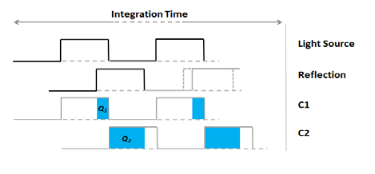
\includegraphics[width=0.75\linewidth]{./images/impulseToF.png}
			\centering
			\caption{Приказ на мерниот протокол на директен ToF од \cite{tofwhitepaper}}
			\label{fig:impulseToF.png}
			\end{figure}

	     \subsubsection{Имплицитен ToF}
		Методата на имплицитен ToF (наречен \textit{Continuous Wave ToF} на англиски) се разликува од директниот на еден клучен начин: Имплицитната метода го мери фазното отстапување помеѓу примениот и оддадениот зрак, кој што непрекинато се испраќа, додека директниот метод работи со директно мерење на време и дискретни импулси. Од оваа добиена фазна разлика, потребни се уште неколку пресметки за да се добие време на изминат пат.

		За разлика од начинот на семплирање кај директната метода, имплцитната метода семплира четири пати при секое мерење, со фазно отстапување $90\degree$. Со оваа техника, фазниот агол помеѓу оддаден и рефлектиран бран $\phi$ и од тоа растојанието $d$ следат:

		$$ \phi = atan(\frac{Q_3 - Q_4}{Q_1 - Q_2}) $$
		$$ d = \frac{c}{4\pi f} \phi $$
		Каде што $c$ е брзината на светлината.


		Од тука, следат и пресметките на интезнитетот на пикселот $A$ и нултото отстапување (\textit{bias}-от) $B$:

		$$ A = \frac{\sqrt{(Q_1 - Q_2)^2  + (Q_3 - Q_4)^2}}{2} $$
		$$ B = \frac{Q_1 + Q_2 + Q_3 + Q_4}{2} $$


		\begin{figure}[H]
			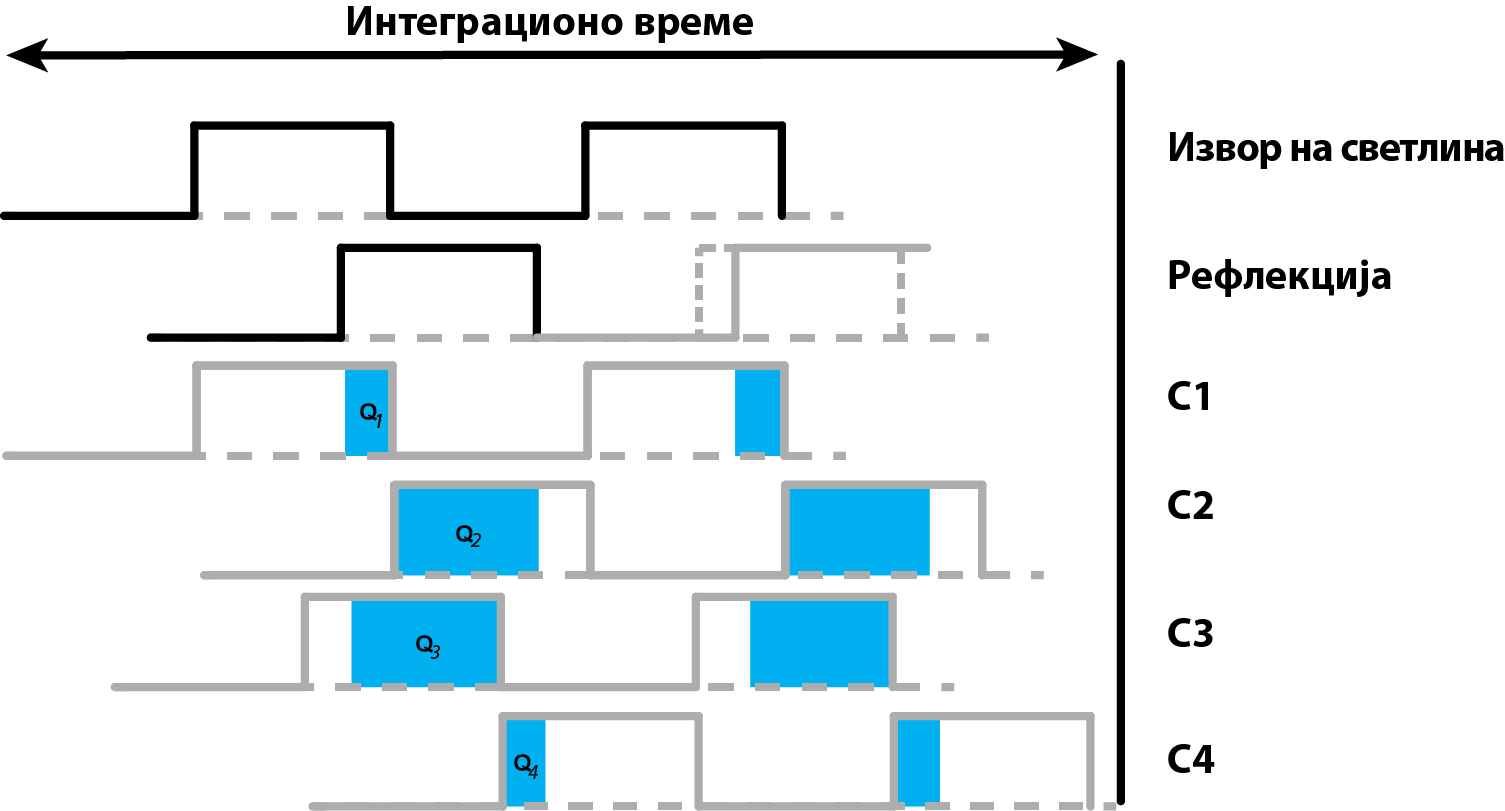
\includegraphics[width=0.75\linewidth]{./images/CWToF.png}
			\centering
			\caption{Приказ на мерниот протокол на имплицитен ToF од \cite{tofwhitepaper}}
			\label{fig:CWToF.png}
			\end{figure}

		Иако имплицитните равенки се навидум безпотребно сложени, всушност одземачките термини го амортизираат влијанието на нултите отстапувања, додека квоциентот во фазната пресметка ги анулира ефектите од било кои системски или рефлектирани засилувања.\\ %quotient?
		Следната равенка ја опишува варијацијата на пресметана длабинска информација како фунцкија на $A$ и $B$, како и фреквенцијата на оддадената светлина $f$ и модулациониот контраст $c_d$, каде што модулационен контраст е способноста на сензорот да ги разделе фотоелектроните - односно чистота на отчитувањето на секој пиксел:

		$$ \sigma = \frac{c}{4\sqrt{2\pi f}} \cdot \frac{\sqrt{A+B}}{c_d A} $$

		Од равенката може да извлече заклучокот дека надежноста на измерените длабини се подобрува со повиска работна фреквенција, висок модулационен контраст, и при јак светлосен интензитет, додека се влошува прецизноста при високо нулто отстапување.
		\\
		Една многу важна појава која што треба да се земе во предвид е појавата на алиасинг. Бидејќи имплицитната метода се базира на фазни разлики кои се повторуваат, ќе се појави растојание на двосмисленост $d_{dvo}$ кое се дефинира според равенката:

		$$ d_{dvo} = \frac{c}{2f} $$

		Сензорот е неупотреблив на растојанија поголеми од $d_{dvo}$, бидејќи не се разликува измерената вредност $z$ од било која вредност $z + k d_{dvo}\ | \ k \in \mathbb{N}$.

  \subsection{Споредба и Анализа на Kinect-от}
    Табелата \ref{tab:comparison} ги споредува важните карактеристики на двете верзии на Kinect сензорот.
    \begin{table}[H]
      \centering
      \label{tab:comparison}
      \begin{tabular}{||c|c|c||}
        \hline
        \textbf{Oсобина} & \textbf{Kinect v1} & \textbf{Kinect v2} \\
        \hline
        Бојна Камера & 640 x 480 (30Hz) & 1920 x 1080 (30Hz) \\
        \hline
        Длабинска Камера & 320 x 240 & 512 x 424 \\
        \hline
        Максимална Длабина & ~4.5M & ~4.5M \\
        \hline
        Минимална Длабина & 40cm & 50cm \\
        \hline
        Хоризонтално Видно Поле & $57\degree$ & $70\degree$ \\
        \hline
        Вертикално Видно Поле & $43\degree$ & $60\degree$ \\
        \hline
        Мотор за Аголно Помесетување & Да & Не \\
        \hline
        Зголбна Резолуција & 20 зглобови & 26 зглобови \\
        \hline
        Истовремено детектирани скелети &  2 & 6 \\
        \hline
        USB стандард & 2.0 & 3.0 \\
        \hline
        Оперативен Систем & $\geq$ Win7 & $\geq$ Win8 \\
        \hline
        Цена (USD) & 50 & 200 \\
        \hline
      \end{tabular}
      \end{table}

    Во текот на истражувањето за Kinect-от, наминавме на неколку трудови и статии во кои се дискутира темата на временската ненадежност поради загревање на Kinect-от при долготрајна употреба. Трудови како \cite{heatup} покажуваат варијација на растојанието измерено од Kinect-от во максимален опсег од приближно 4 милиметри.

    \begin{figure}[H]
      \centering
      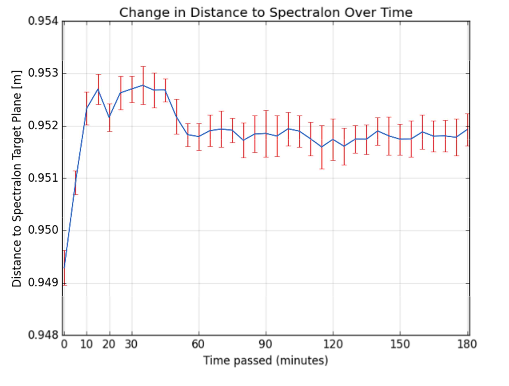
\includegraphics[width = 0.75\linewidth]{./images/heatup.png}
      \label{fig:heatup}
      \caption{Мерења од страна на Џереми Стјуард \cite{heatup}}
    \end{figure}

    Изведовме три слични тестирања на три различни денови, и ги добивме следните резултати:

    \begin{figure}[H]
      \centering
      \begin{minipage}{0.45\linewidth}
        \centering
        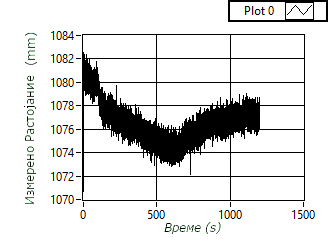
\includegraphics[width = \textwidth]{./images/kinect_graph_1_mk.png}
      \end{minipage}
      \begin{minipage}{0.45\linewidth}
          \centering
          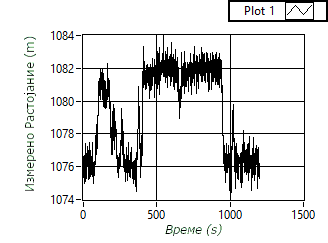
\includegraphics[width = \textwidth]{./images/kinect_graph_2_mk.png}
        \end{minipage}
      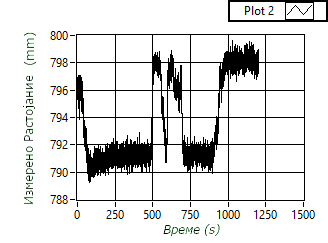
\includegraphics[width = 0.45\linewidth]{./images/kinect_graph_3_mk.png}
      \caption{Наши испитувања на варијација на отчитување според време}
      \end{figure}

    На крај нашите испитувања открија стохастична варијација на отчитувањата во опсег од приближно 10 милиметри. Нашата задача не е одговорна и нема посебно барање за милиметарска прецизност, односно резултатите се сепак задоволителни.

\newpage

\section{Алгоритам за препознавање}

  Постојат неколку различни компоненти кои што го прават Kinect-от пробив во технологијата. Хардверот е добро дизајниран и ја извршува својата функција при што има прифатлива цена. Меѓутоа, штом вниманието се тргне од брзото мерење на растојание, тоа се фокусира на методот за следење на тела. Во овој случај тој претставува класична техника за препознавање шеми која што е карактеристично имплементирана.\bigbreak

	Претходните уреди за следење на тела имаат недостаток - за да го следат телото, човекот мора да застане во калибрациона поза за да се овозможи употреба на алгоритам за барање усогласеност во делови од сликата. Од тука се користи логиката дека ако раката на телото се наоѓа во одреден регион во првата слика, тогаш во наредната слика таа рака нема нема да може да се има задвижено далеку од претходниот регион, и само се бара усогласување во близина на тој регион.\bigbreak

	Иако логиката е добра, се јавува проблем доколку се изгуби локацијата на телото за било која причина, доколку објект кој и само за момент го попречи телото кое што се следи. Следењето на поголем број на тела значително ја отежнува работата, и доколку се изгуби следењето на некое тело, тоа тешко може да се врати.\bigbreak

	Тоа што го прави Kinect-от не е следење на веќе препознаено тело, туку лоцирање на делови од телото со локална анализа на секој пиксел од сликата. Како што се опишува во \cite{machinelearning}, традиционалното препознавање на шеми работи преку тренирање на одлучувачка структура (со користење на машинско учење) со голем број на примероци на објектот кој што треба да го препознае. Тренирањето на одлучувачката структура се изведува со доведување на голем број на мерења од т.н. „особини“ на класификатор кои што треба да содржат потребни информации за препознавање на објектот, при што најчесто тешкиот дел е одредувањето на особините кои што треба да се мерат.\bigbreak

	Овие особини се базирани на едноставна формула:

  \begin{equation} \label{eq:depth}
	  f_\theta(I,\textbf{x}) = d_I(\textbf{x}+\frac{\textbf{u}}{d_I(\textbf{x})}) - d_I(\textbf{x}+\frac{\textbf{v}}{d_I(\textbf{x})})
    \end{equation}
  \\
  каде што $d_I(\textbf{x})$ е длабочината, односно растојанието од Kinect-от кај пикселот \textbf{x} во слика $I$, и параметрите $\theta = (\textbf{u},\textbf{v})$ ги опишуваат офсетите (offsets) \textbf{u} и \textbf{v}.

  \begin{figure}[H]
	  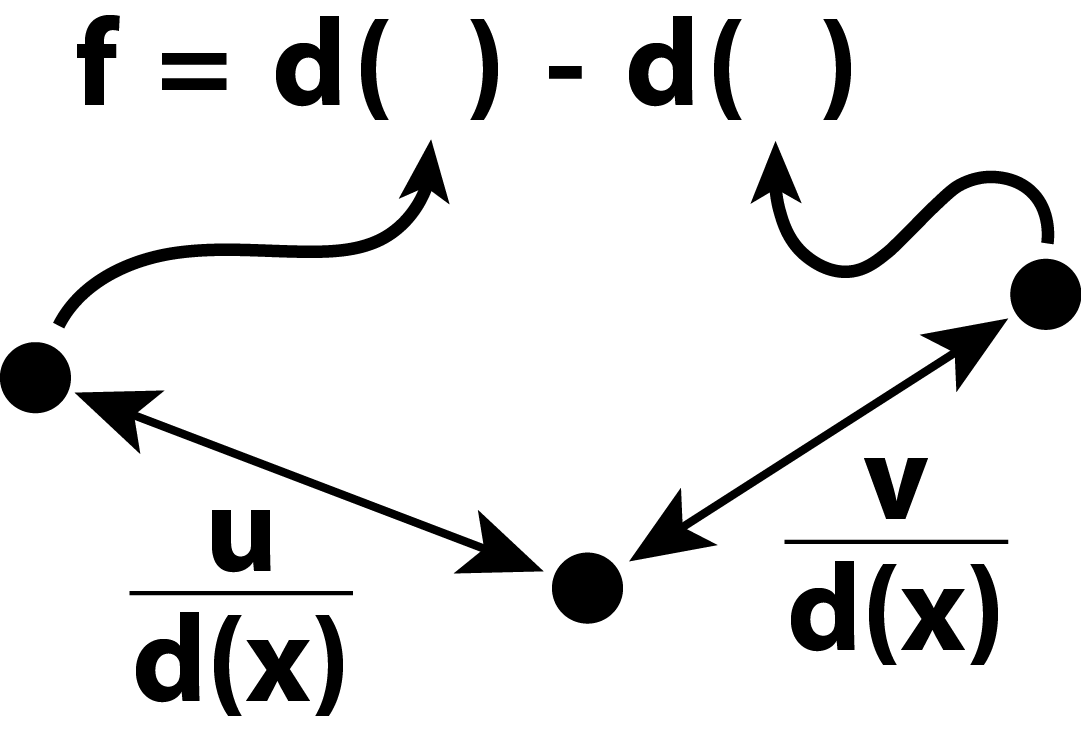
\includegraphics[width=0.35\linewidth]{./images/kinectfeature.png}
		\centering
		\caption{Репрезентација на горенаведената формула од \cite{machinelearning}}
		\label{fig:kinectfeature.png}
	  \end{figure}

	Во формулата, поместувањето (offset) се дели со $d_I(\textbf{x})$ со цел да се направи независно од длабочината, а истовремено да се зголемува или намалува во зависност од големината на објектот. Како излез од $f$ добиваме информации за 3D обликот на просторот околу разлгледуваниот пиксел $x$.\bigbreak

  На сл. \ref{fig:depth_features.png} се прикажани две особини за различни пиксел локации \textbf{x}. Особината $f_{\theta_1}$ гледа нагоре од каде равенката \ref{eq:depth} ќе даде голема позитивна вредност за пиксели \textbf{x} во близина на врвот на телото, но за пиксели \textbf{x} во пониска локација на телото ќе даде вредност блиску до нула. Од друга страна особината $f_{\theta_2}$ може да се користи за одредување на тенки вертикални структури, како на пример рацете.

  \begin{figure}[H]
    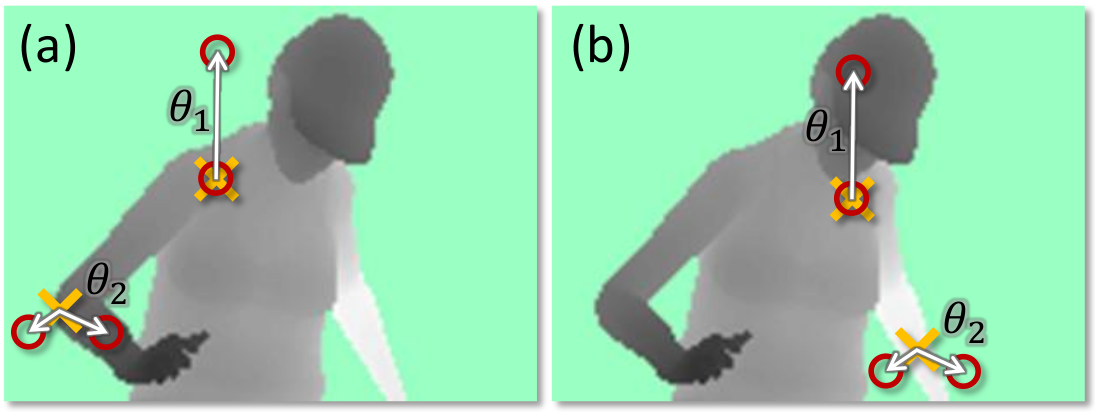
\includegraphics[width=0.75\linewidth]{./images/depth_features.png}
    \centering
    \caption{Особини на длабинската слика од \cite{machinelearning}}
    \label{fig:depth_features.png}
    \end{figure}

  Бидејќи ова не е доволно за да се одреди дали објект е еден екстремитет или друг, се применува машинско учење.

  %	\subsection{Машинско учење}
	Машинско учење претставува наука која се занимава со постигнување на посаканото однесување на компјутери без дирекнто наредбено програмирање. Во минатата деценија, машинското учење имаат овозможено автономни возила, практично препознавање на говор, ефективно пребарување на интернет, и значително подобрено познавање на човечкиот геном. Машинското учење во денешно време е толку продорно што луѓето го користат десетици пати дневно без тоа да го знаат. Многу научници исто сметаат дека тој е најдобриот начин за правење напредок кон вештачка интелигенција која е на ниво на човек.

	Задачите на машинско учење во главно се класифицирани во две пошироки категории, во зависност од тоа дали има влезен „тренинг“ сигнал или повратна врска доведена во системот за учење:

	\begin{itemize}
		\item \textit{Надгледувано учење}\\Компјутерот добива пример влезови и нивни посакани излези, кои што се дадени од „учител“, и целта е да научи генерално правило кое што пресликува влезови на излези.
    \begin{itemize}
      \item \textit{Полу-надгледувано учење}\\Компјутерот добива нецелосен тренинг сигнал: множество на тренинг елементи од кои недостасуваат неколку (често повеќе) посакувани излези.
      \item \textit{Активно учење}\\Компјутерот може да добие именувани информации само од ограничен број на тренинг примери (базирано на буџет), и исто така мора да го оптимизира својот избор на објекти за кои ќе добива именувани информации. При негово користење во интерактивна средина можно е да ги презентира на корисникот за именување.
      \item \textit{Засилено учење}\\Компјутерот добива информации (во форма на награди или казни) само преку повратна врска. Видот на информации зависи од акциите на програмата во динамичка средина, како на пример управување на возило или игра со противник.
      \end{itemize}
		\item \textit{Ненадгледувано учење}\\Компјутерот не добива именувани информации, односно се остава алгоритамот за учење сам по себе да пронајде структура по која ќе ги групира влезовите.
    \end{itemize}

  Алгоритам за машинско учење кој што пресликува податоци во соодветна категорија се нарекува класификатор (Classifier). Еден пример за класификатор е т.н. „дрво на одлучување“. дрво на одлучување претставува алат за поддшка на одлучување кое користи дијаграм или модел во форма на дрво, составено од одлуки и нивни можни последици.\\
  Во Kinect-от се користи „шума на одлучување“ што всушност претставува збир на поголем број дрва. Секое дрво се тренира на неколку особини користејќи длабински слики кои имаат претходно означени делови од телото, се додека не дава точни класификации за одреден дел од телото за повеќе тест слики.

  Овие тренирани класификатори доделуваат вредост за веројатност, односно колку сигурни се дека тој пиксел припаѓа на одреден дел од телото, а наредниот алгоритам ги избира најверојатните области за секој различен дел од телото. Според тоа, одредена површина пиксели ќе биде сместена во категоријата „рака“ ако класификаторот за препознавање на раце има најголема вредност за веројатност во таа област во споредба со другите класификатори за различни делови на телото. Последниот чекор се состои од цртање на претпоставени локации на соодветни врски(joints) во тие области.

  \begin{figure}[H]
    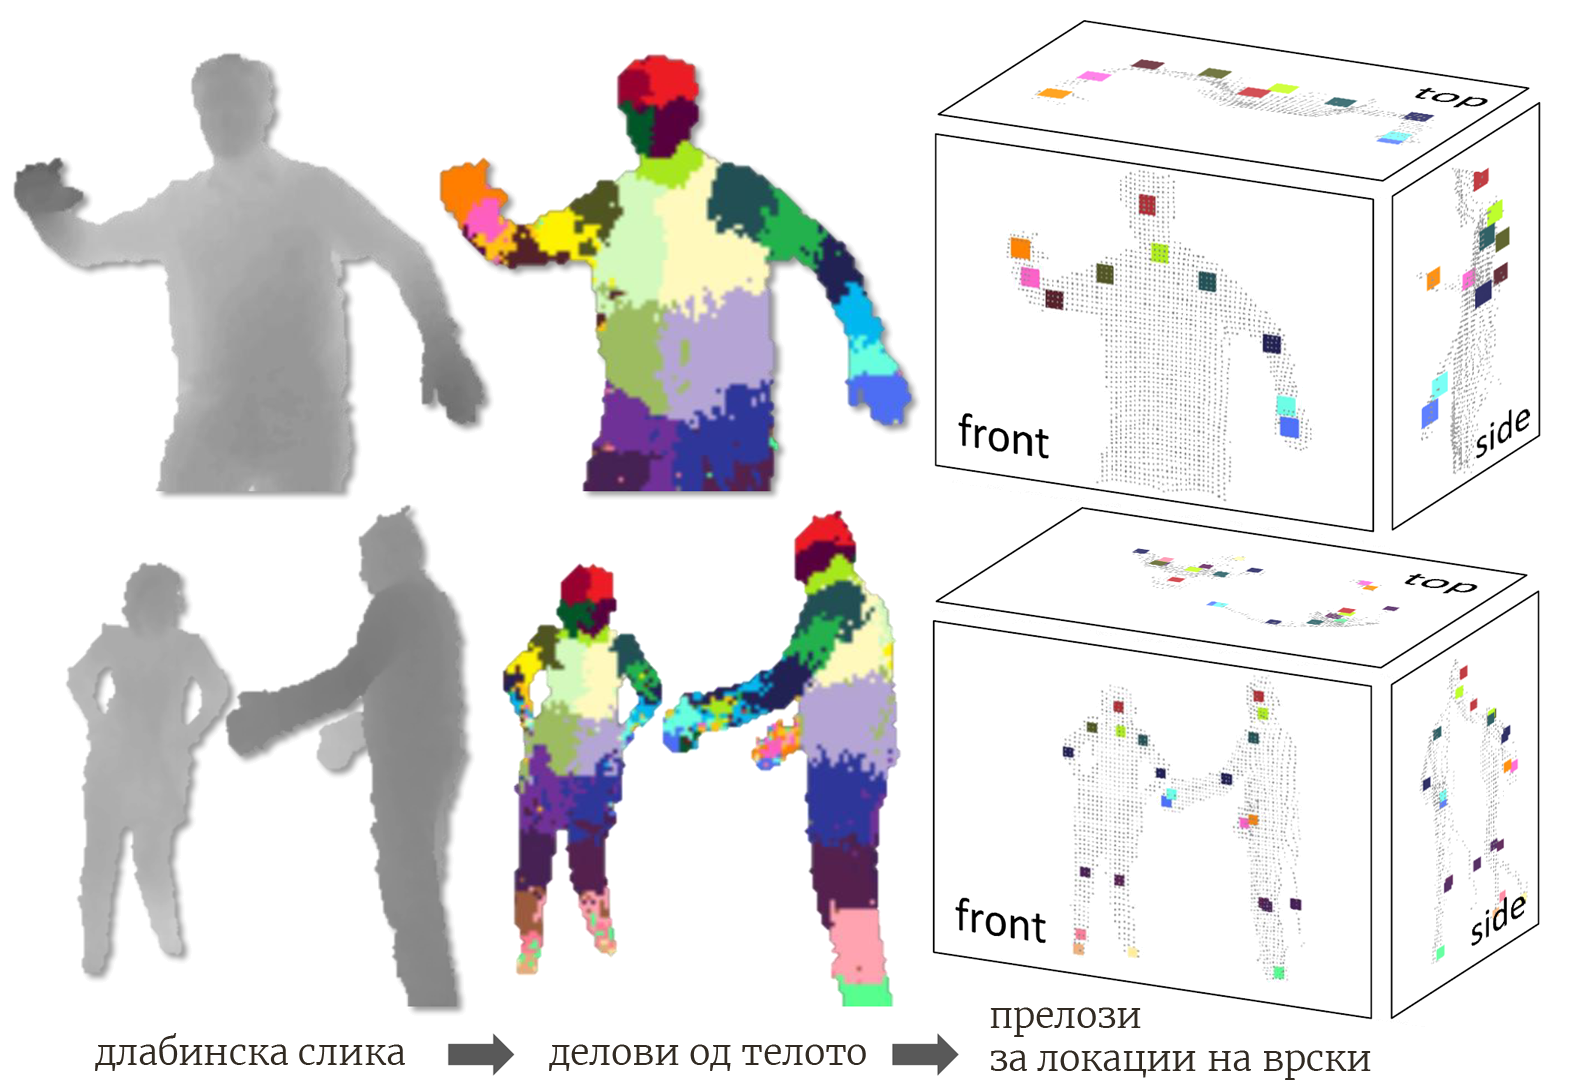
\includegraphics[width=0.75\linewidth]{./images/bodyparts.png}
    \centering
    \caption{Алгоритам за препознавање од \cite{machinelearning}}
    \label{fig:bodyparts.png}
    \end{figure}

  Бидејќи пресметката користи само длабински информации за три пиксели и може да се обработи од страна на GPU-то, системот може да работи со 200 слики во секунда (fps) и нема потреба од калибрациона поза. Секоја слика се обработува посебно поради што нема следење и нема опасност од губење на локацијата на телото, по што мора да се повтори калибрационата поза, и исто така постои можност за следење на поголем број на тела истовремено.

\newpage

\section{Примери од SDK-то на Kinect-от} \label{sec:example}
  Ова поглавје се состои од два делови: еден општ пример во C++ што ќе служи за опис на начинот на отчитување од Kinect-от, а во вториот дел ќе се прикажани неколку слики што се добиваат на излез од примерните програми зададени во SDK-то (Software Development Kit) за Kinect, како и кратки описи на другите можности на SDK-то.

  \subsection{Начин на отчитување во C++}
    Програмирањето на Kinect-от, односно неговото отчитување, не е сосема едноставно, туку неколку чекори се потребни за да се стигне до добивањето на самата слика.

    \begin{figure}[H]
      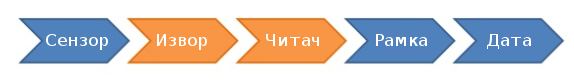
\includegraphics[width=0.75\linewidth]{./images/programming_flow_trimmed.png}
      \centering
      \caption{Општ протокол за отчитување на Kinect-от}
      \label{fig:programming_flow_trimmed.png}
      \end{figure}

    Причината за оваа сложеност е поради големата количина на можности пружена од интерфејсот за програмирање од Microsoft. За секој член од отчитувачкиот процес постои барем една опција која би влијаела на крајната слика.

    Со следната програма се детектираат до 6 луѓе, и врз нивните тела се цртаат точки во сите 26 пресметани зглобови. Истовремено се испраќа состојбата на нивните раце и се прикажува таа состојба со обоени кругови околу рацете. Бојата се менува во зависност од тоа дали тие се отворени, затворени, или во „лассо“ состојби (два кренати прсти). Секој од зглобовите има свои координати во декартов систем со центар во средината на самиот Kinect. Пристапот употребен во овој пример е инспириран од примерите дадени и од Microsoft и од Nancy Owen \cite{nancyowen}.
    \begin{verbatim}
          #include "stdafx.h"
          #include <iostream>
          #include "util.h"
          #include <thread>
          #include <chrono>
          #include "ppl.h"
          #include "Kinect2_Tools.h"
          int main(int argc, char ** argv){
            try {
                Kinect kinect;
                kinect.initializeSensor();
                kinect.initializeColor();
                kinect.initializeBody();

                while(true){
                  kinect.updateColor();
                  kinect.updateBody();
                  kinect.drawColor();
                  kinect.drawBody();
                  kinect.showBody();
                }

                 }
            catch (std::exception &except)
            {
              std::cout << except.what() <<std::endl;
            }
          }
        \end{verbatim}

    Кодот е скратен со помош на фунцкиите кои сe напишани и вградени во проектот преку \verb+include "Kinect2_Tools.h"+ и \verb+Kinect2_Tools.cpp+ фајловите. Во анекс II е прикачен линк кон целосниот проект на Github, кој слободно може да се спушти, промени, и прошири.

  \subsection{Примери од SDK-то}
     Примерите дадени во SDK-то се разновидни, и пружат моќни можности. Најосновниот пример е препознавање на скелет и неговото прикажување:
     \begin{figure}[H]
      \centering
      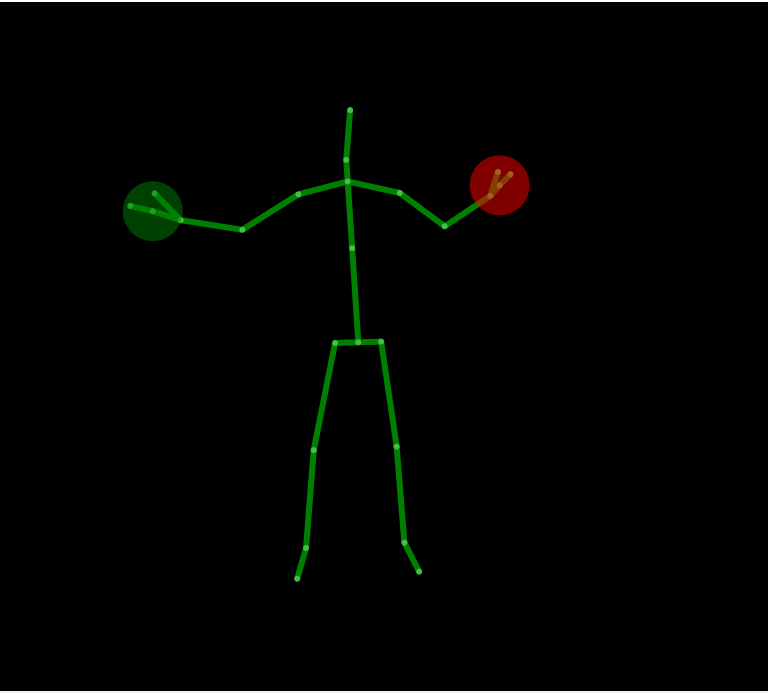
\includegraphics[width = 0.75\linewidth]{./images/shrug_for_windows.png}
      \label{fig:shrug}
      \caption{Детектиран скелет со прикажана отворена лева рака и затворена десна рака}
    \end{figure}

    SDK-то содржи примери кои го употребуваат препознавањето за посложени задачи како што се тродимензионална реконструкција и постигнување ефект на зелена завеса (\textit{green screen}). Исто содржи и програми што ги користаат другите способности на API-то - препознавање на гестикулации и на лицето, и на рацете, а дури и препознавање на говор е можно со помош од соодветните пакети од Microsoft.

    \begin{figure}[H]
      \label{fig:happy_no}
      \centering
      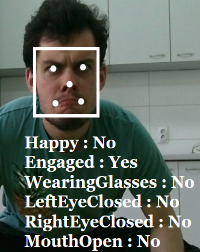
\includegraphics[width = 0.25\linewidth]{./images/happy_no_small.png}
      \caption{Препозанвање на расположеност, заинтересираност, и други карактеристики на лицето}
    \end{figure}

\newpage

\section{DaNI}
  \begin{figure}[H]
    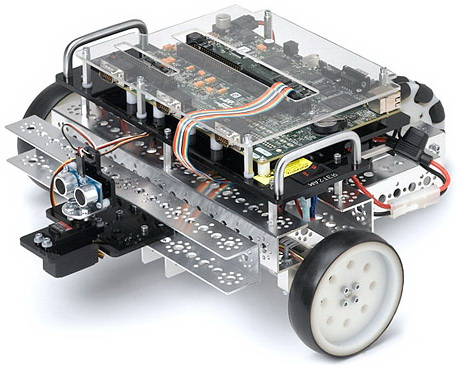
\includegraphics[width=0.6\linewidth, keepaspectratio]{./images/dani_isometric.jpg}
    \centering
    \caption{Роботот DaNI}
    \label{fig:dani_isometric}
    \end{figure}

	National Instruments (NI) LabVIEW комплетот за роботика се состои од DaNI 2.0 (сл.\ref{fig:dani_isometric}), кој содржи:

	\begin{itemize}
		\item Pitsco Education 12 VDC мотори со 152 rpm и 21.6 kg-cm вртежен момент
		\item Оптички квадратурни енкодери со 400 импулси при револуција
		\item PING))) ултразвучен сензор за мерење на растојанја помеѓу 2cm и 3m
		\item PING))) монтажен држач за работен агол од $180 \degree$
		\item Два Pitsco Education TETRIX 10.16cm тркала и едно омни тркало за насочување
		\item sbRIO единица и соодветни кабли за поврзување
		\end{itemize}

	Хардверот може да биде проучуван, обратно инжениран, и модифициран од студенти. Меѓутоа, главната цел е роботска перцепција и контрола кои се имплементирани во LabVIEW софтвер развиен на одделен сервер (компјутер) и спуштен на роботскиот компјутер.

	\begin{figure}[H]
		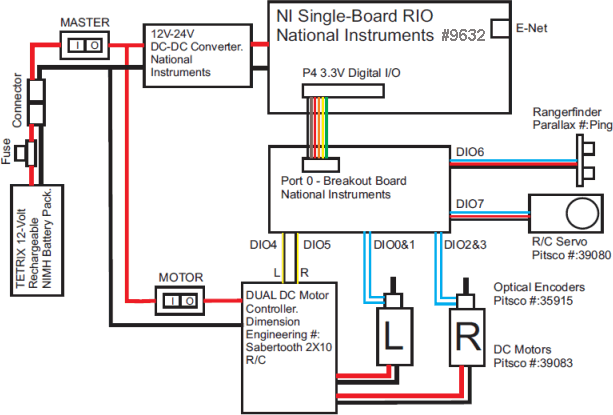
\includegraphics[width=0.75\linewidth]{./images/dani_block_diagram.png}
		\centering
		\caption{Блок дијаграм на DaNI}
		\label{fig:dani_block_diagram.png}
		\end{figure}

	\subsection{Актуатори}
		Од страната на актуатори, DaNI поседува два DC мотори со вградени редуктори, и еден серво мотор. DC моторите се користат за движење на роботот, а серво моторот има улога прецизно да го ротира PING))) ултразвучниот сензор. Подолу се наведени нивните карактеристики.

	  \subsubsection{DC мотори}
		  DC мотор со четкици претставува внатрешно комутиран електричен мотор дизајниран да биде напојуван со извор на еднонасочна струја. Неговата брзина може да се менува со промена на работниот напон или јачината на магнетото поле.
		  Во DaNI се применети два DC мотори, поточно TETRIX MAX DC мотори(сл.\ref{fig:dc_motor_iso.png}).

		  \begin{figure}[H]
    	  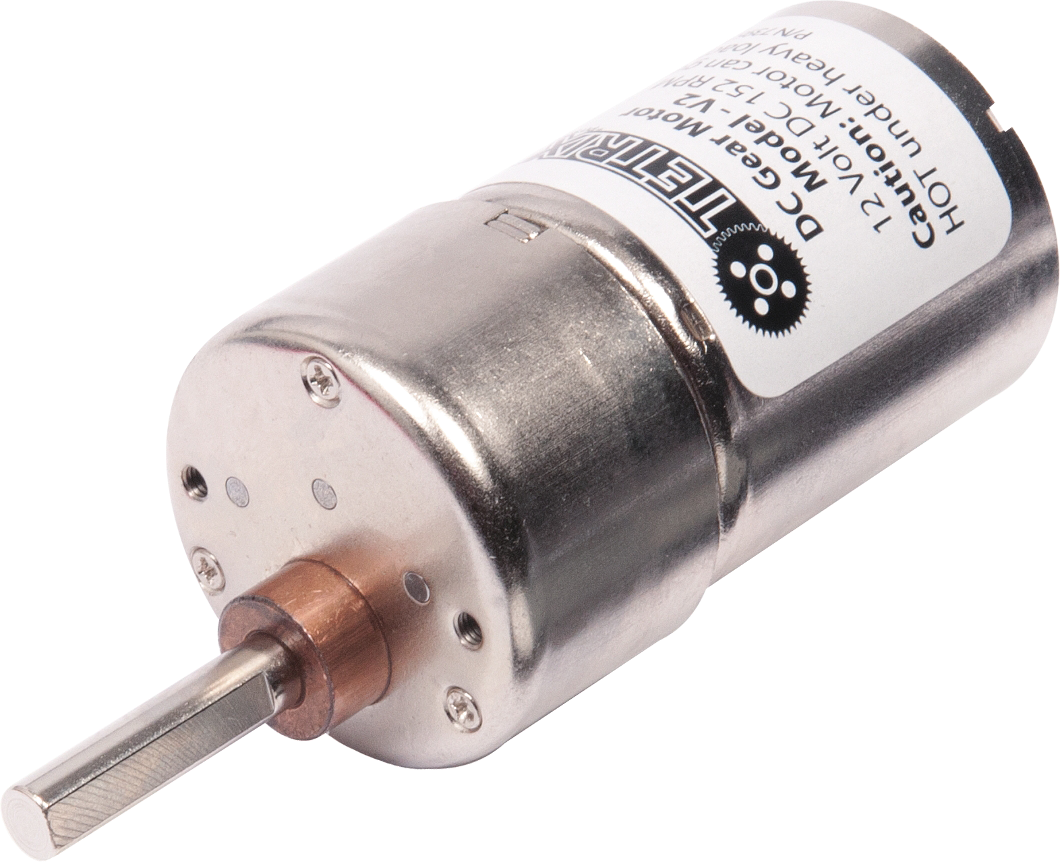
\includegraphics[width=0.35\linewidth]{./images/dc_motor_iso.png}
			  \centering
			  \caption{Tetrix Max DC мотор}
			  \label{fig:dc_motor_iso.png}
			  \end{figure}

      \begin{table}[h]
        \caption{Карактеристики на DC моторите}
        \label{tab:dcmotor}
        \begin{center}
          \begin{tabular}{||c|c|c||}
            \hline
            \textbf{При нормални услови:} & & \\
            \hline
             & Номинален Напон & $6-13.8V$\\
             & Температура на Околина & $-10 \pm 60 \degree C$\\
            \hline
            \textbf{Услови на Испитување:} & & \\
            \hline
            & Напон & $12V$ \\
            & Температура на Околина & $28 \degree C$\\
            & Влажност на Воздухот & $44\% Рел.$\\
            \hline
            \textbf{Електрични Особини:} & & \\
            \hline
            \textbf{Неоптоварен:} & & \\
            \hline
            & Брзина & $150 \pm 10 \ vrt/s$ \\
            & Струја & $0.34А\ (0.68A max.)$ \\
            \hline
            \textbf{Оптоварен:} & &\\
            \hline
            & Вртежен Момент & $0.382Nm $\\
            & Струја & $0.91А (1.37А max.)$\\
            & Брзина & $137.5 \pm 10 \%\ vrt/s$\\
            \hline
          \end{tabular}
        \end{center}
      \end{table}


		\begin{comment}  \renewcommand{\theenumii}{\arabic{enumii}}
        \renewcommand{\theenumiii}{\arabic{enumiii}}
	      \begin{enumerate}
        \item При нормални услови на работа:
          \begin{enumerate}
            \item Номинален напон: $ 6-13.8 V $
					  \item Температура на околината: $ -10 \pm 60 \degree C $
					  \item Насока на ротација: Спротивно од стрелката на часовникот\\Позитивен пол поврзан со црвен „+“\\Негативен пол поврзан со „-“\\Гледајќи кон оската на излезното вратило
					  \end{enumerate}
		    \item Услови на испитување:
          \begin{enumerate}
            \item Напон: DC 12 V
            \item Температура на околината: $ 28 \degree C $
            \item Влажност на воздухот: 44 \% RH
            \item Испитуваниот уред е поставен хоризонтално
            \end{enumerate}
	  	  \item Електрични способности(По 30 секунди напојување)
        	\begin{enumerate}
            \item Без оптоварување
              \begin{enumerate}
                \item Брзина: 150 $\pm$ 10 RPM
                \item Струја: 0.34А (0.68А max)
                \end{enumerate}
				    \item Со оптоварување
              \begin{enumerate}
                \item Вртежен момент: 3.9kg.cm
                \item Струја: 0.91А (1.37А max)
                \item Брзина: 137.5 $\pm$ 10 \% RPM
                \item Вртежен момент на запирање: /
                \item Струја на запирање: /
                \end{enumerate}
            \end{enumerate}
	      \item Механички карактеристики
          \begin{enumerate}
            \item Аксијално поместување на вратилото: $\leq$ 0.5mm
            \end{enumerate}
        \item Својства на моторот:
          \begin{enumerate}
            \item Струја без оптоварување: 0.19А
            \item Брзина без оптоварување: 11000 $\pm$ 10 \% RPM


            \end{enumerate}
        \end{enumerate}
      \end{comment}

		  Двата DC мотори присутни во конструкцијата се контролирани со помош на Sabertooth Dual 10A Motor Driver. Тој може да напојува два DC мотори со четкици со струја до 10А поединечно, со максимални 15А за кратки временски периоди, со многу тивка операција поради ултрасоничната брзина (32kHz) на контрола на неговите транзистори. Sabertooth исто така претставува првиот синхрон регенеративен мотор драјвер во својата класа. Регенеративната топологија значи дека батериите на уредот се полнат кога на уредот му се наредува да забави или да се врати назад, при што исто така ја зголемува и брзината на реакција. Вклучува внатрешно напојување од 5V кое може да напојува микроконтролер или R/C приемник.

		  Наредно се зададени техничката скица(сл.\ref{fig:motor_schematic.png}) на моторот со неговите димензии, како и графикот на карактеристики на моторот за различно оптоварување(сл.\ref{fig:motor_graph.png}). Овој график ги дава целокупните карактеристики, т.е. карактеристиките на моторот заедно со редукторот.

      \begin{figure}[H]
        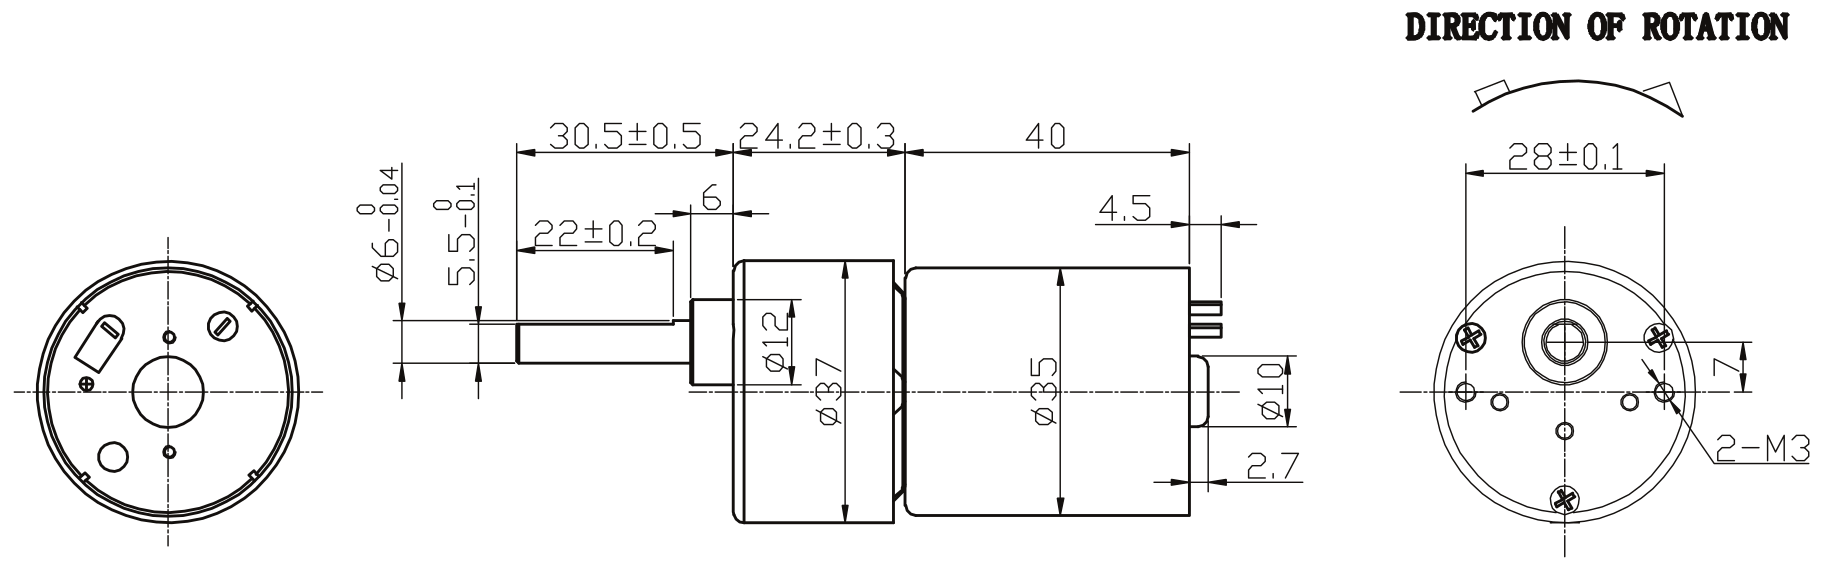
\includegraphics[width=0.75\linewidth]{./images/motor_schematic.png}
		    \centering
        \caption{Техничка скица на DC моторот}
		    \label{fig:motor_schematic.png}
		    \end{figure}

	    \begin{figure}[H]
		    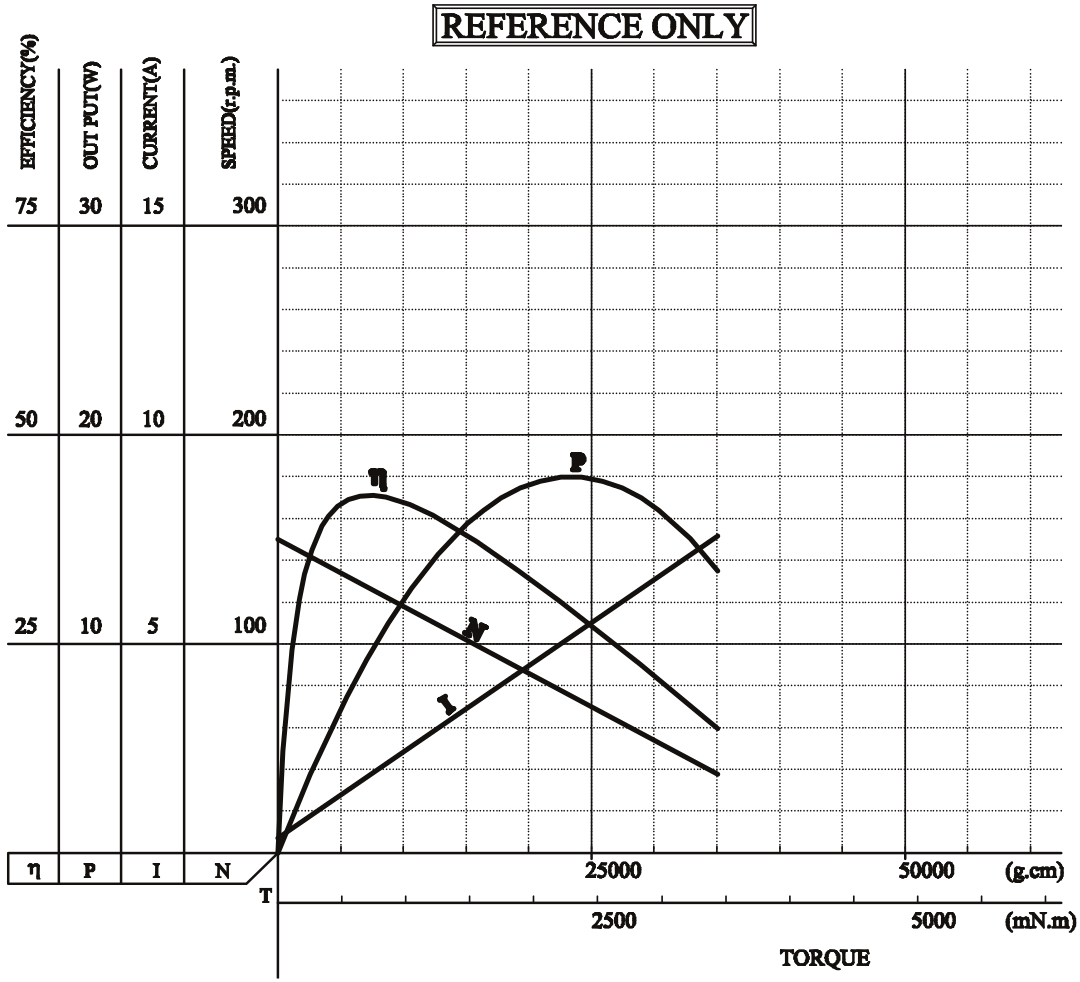
\includegraphics[width=0.75\linewidth]{./images/motor_graph.png}
		    \centering
		    \caption{Карактеристични вредности на DC моторот}
		    \label{fig:motor_graph.png}
	      \end{figure}

    \subsubsection{Серво мотор}
      Серво мотор е ротационен актуатор кој дозволува за прецизна контрола на аголна позиција. Тој се состои од мотор поврзан со сензор за повратни информации за позиција. Исто така има потреба од серво драјвер, кој прима команден сигнал од контролен систем, го засилува сигналот, и пренесува електрична струја до серво моторот со цел да произведе движење пропорционално со командниот сигнал. За оваа цел го користи и сензорот за повратни информации за позиција за да се добие прецизна контрола на ротационата позиција на моторот. Ова е т.н. систем со затворена повратна врска.

      Единствена функција на серво моторот во оваа конструкција е ротација на PING))) сензорот, поради што тој не е изложен на значителни оптоварувања.

      \begin{table}[h]
        \caption{Карактеристики на серво моторот}
        \label{tab:servomotor}
        \begin{center}
          \begin{tabular}{||c|c||}
            \hline
            Димензии & 39.88 х 19.81 х 37.85mm\\
            \hline
            Тежина & 45g\\
            \hline
            Ранг на напон & 4.8V - 6.0V\\
            \hline
            Брзина без оптоварување (4.8V) & 0.22sec/60\degree\\
            \hline
            Брзина без оптоварување (6.0V) & 0.18sec/60\degree\\
            \hline
            Вртежен момент на запирање (4.8V) & 4.8kg.cm\\
            \hline
            Вртежен момент на запирање (6.0V) & 6.0kg.cm\\
            \hline
            Максимален ранг на PWM & 553-2425\micro sec\\
            \hline
            Поминат агол по \micro sec & .102\degree/\micro sec\\
            \hline
            Максимален пат & 190.5\degree \\
            \hline
            Амплитуда на импулс & 3-5V \\
            \hline
            Работна температура & -20\degree C до +60\degree C \\
            \hline
            Потрошувачка на струја - неактивен (4.8V) & 8mA \\
            \hline
            Потрошувачка на струја - неактивен (6V) & 8.8mA \\
            \hline
            Потрошувачка на струја - без оптоварување (4.8V) & 150mA \\
            \hline
            Потрошувачка на струја - без оптоварување (6V) & 180mA \\
            \hline
            Можност за континуирана ротација & + \\
            \hline
            Насока со зголемување на PWM сигнал & Во насока на часовата стрелка \\
            \hline
            Вид на запченици & Запченици со прави заби \\
					  \hline
            Материјал на запченици & Карбонит \\
            \hline
            \end{tabular}
          \end{center}
        \end{table}

		  \begin{figure}[H]
        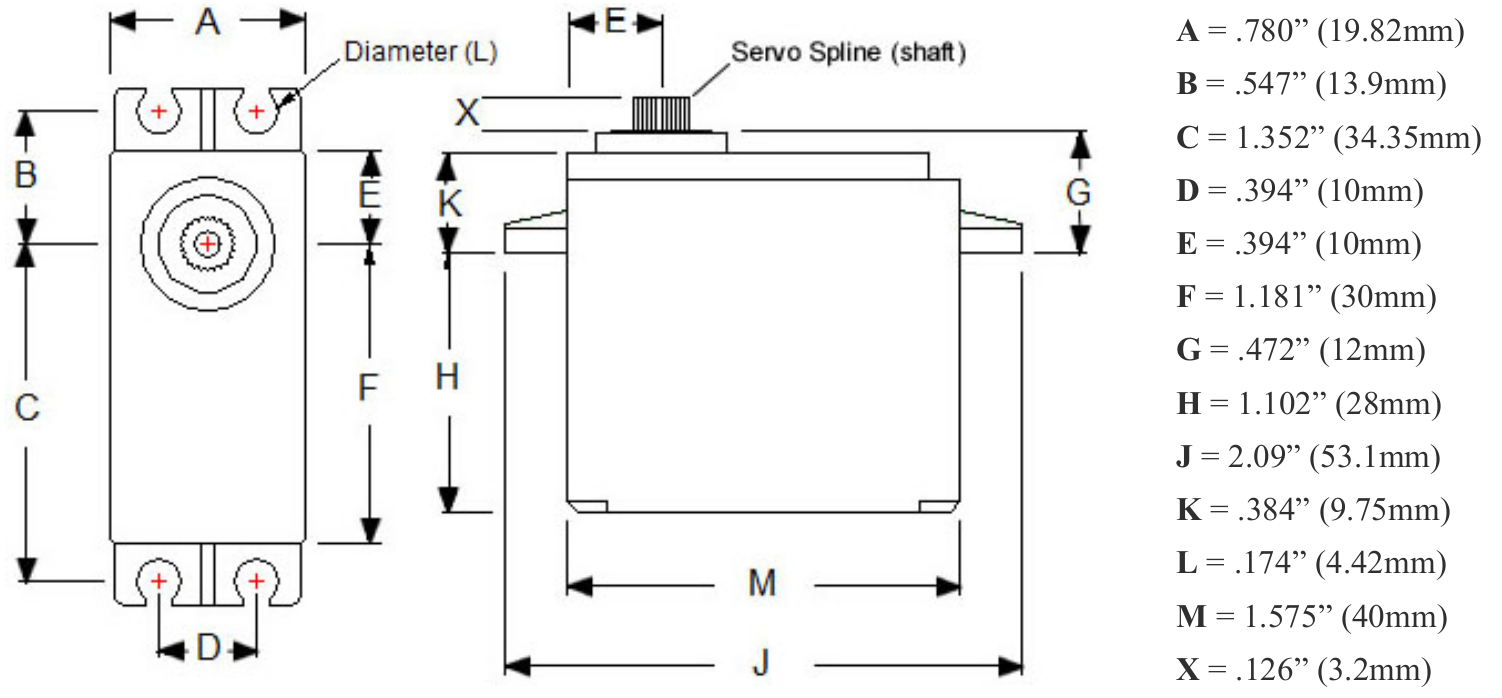
\includegraphics[width=0.75\linewidth]{./images/servo_schematic.png}
        \centering
        \caption{Димензии на серво моторот}
        \label{fig:servo_schematic.png}
        \end{figure}

    \subsubsection{PWM}
    	PWM (Pulse Width Modulation) е начин на аналогно управување базиран на употребата на чисто дигитални сигнали. При една претходно одредена фреквенција, имаме една соодветна периода, $T(s)$. Во рамките на една периода, можеме да ја дефинираме врската помеѓу времетраењето на активноста (ОN) и времетраењето на неактивноста (OFF) на еден дигитален излез. Добиениот „аналоген“ излез (ефективниот напон) се пресметува со следната равенка:\\

      $$ V_{PWM} = V_{dig} \cdot \frac{T_{ON}}{T_{ON} + T_{OFF}} = V_{dig} \cdot \frac{T_{ON}}{T} $$

      На пример, ако имаме работна фреквенција 20kHz, имаме периода $50\mu s$. Нека дигиталниот излез биде 5V (т.е. ON = 5V, OFF = 0V). Ако за $30\mu s$ од секоја периода задаваме ON сигнал, а за останатите $20\mu s$ задаваме OFF сигнал, на излез ќе го добиеме ефективен напон:

      $$ V_{PWM} = 5 \cdot \frac{30}{30+20} = 5 \cdot 0.6 = 3V $$

  \subsection{Сензори}
    Во најширока дефиниција, сензор претставува уред, модул или подсистем чија задача е да препознае настани или промени во својата околина, и да испрати согласна информација кон останатата електроника (најчесто компјутерски процесор).

    Во DaNI употребуваме два вида на сензори: енкодер и ултразвучен сензор.

    \subsubsection{Енкодер}
      Ротационен енкодер е електромеханички уред кој ја претвора аголната позиција или движење на вратило во аналоген или дигитален сигнал.

		  Постојат два главни видови: апсолутни и инкрементални (релативни). Излезот од апсолутни енкодери ја изразува моменталната позиција на вратилото, што ги прави аголни трансдусери. Излезот на инкрементални енкодери дава информација за \textit{движењето} на вратилото кое понатаму се процесира во информации како за брзина, растојание и позиција.

		  Ротационите енкодери се користат во многу области на апликации кои имаат потреба од прецизна контрола на неограничена ротација на вратило, вклучувајќи индустриски контрола, роботика, фотографски леѓи за специјални примени, компјутерски влезни уреди, и ротациони радарни платформи.

		  Во нашиот случај, енкодерот е инкрементален квадратурен енкодер(сл.\ref{fig:encoder.png}), што значи дека користи два излеза A и B кои се наоѓаат на 90 \degree фазно поместување еден од друг(сл.\ref{fig:encoder_quadrature.png}).

		  \begin{table}[h]
        \caption{Зголемување на фазата имплицира ротација во насока на стрелките на часовникот}
        \label{tab:fazno}
        \begin{center}
          \begin{tabular}{||c|c|c||}
            \hline
            Фаза & A & B \\
            \hline \hline
            1 & 0 & 0 \\
            \hline
					  2 & 0 & 1 \\
            \hline
            3 & 1 & 1 \\
            \hline
            4 & 1 & 0 \\
            \hline
            \end{tabular}
          \end{center}
        \end{table}

      \begin{figure}[H]
        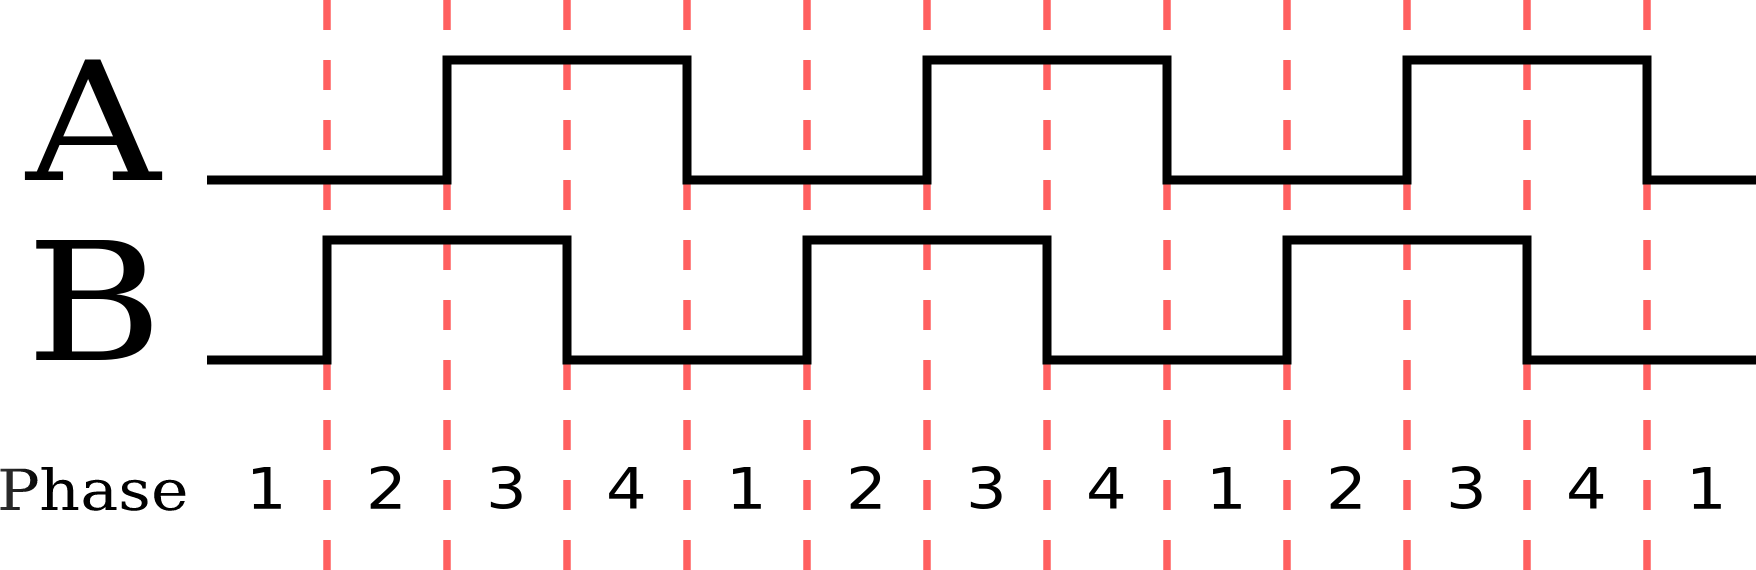
\includegraphics[width=0.5\linewidth]{./images/encoder_quadrature.png}
        \centering
        \caption{Два квадратни бранови во квадратура (ротација во насока на стрелките на часовникот)}
        \label{fig:encoder_quadrature.png}
        \end{figure}

      Исто така дискот има 400 отвори, односно енкодерот има резолуција од 0.9\degree.

      \begin{figure}[H]
        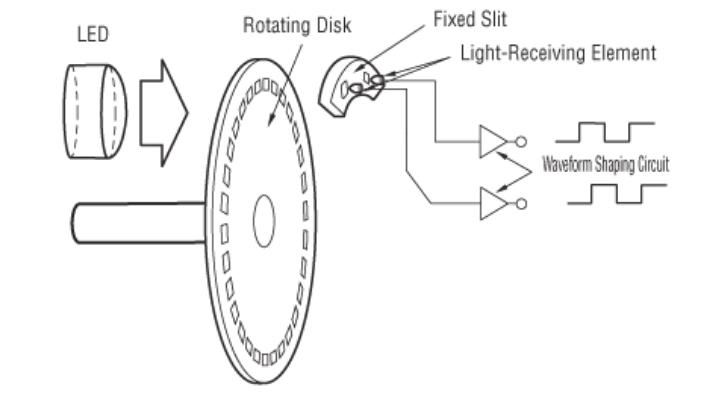
\includegraphics[width=0.5\linewidth]{./images/encoder.png}
        \centering
        \caption{Шема на оптички енкодер}
        \label{fig:encoder.png}
        \end{figure}

    \subsubsection{Ултразвучен сензор}
      Ултразвучниот сензор PING))) од Паралакс(сл.\ref{fig:ping_dims.png}) е способен да извршува прецизни мерења на растојанија од 2cm до 3m. Лесно се приклучува на микроконтролери како BASIC Stamp, Propeller chip, или Arduino, користејќи само еден I/O пин. Се напојува со 5V и 30mA.

		  PING))) сензорот работи со пренесување на ултрасончен (високо над осетливиот ранг на човекот) збир (burst) на бранови, и произведува излезен пулс кој соодветствува на времето потребно за ехото на брановите да се врати до сензорот. Со мерење на ширината на излезниот пулс, лесно може да се пресмета растојанието до објектот.

		  \begin{figure}[H]
        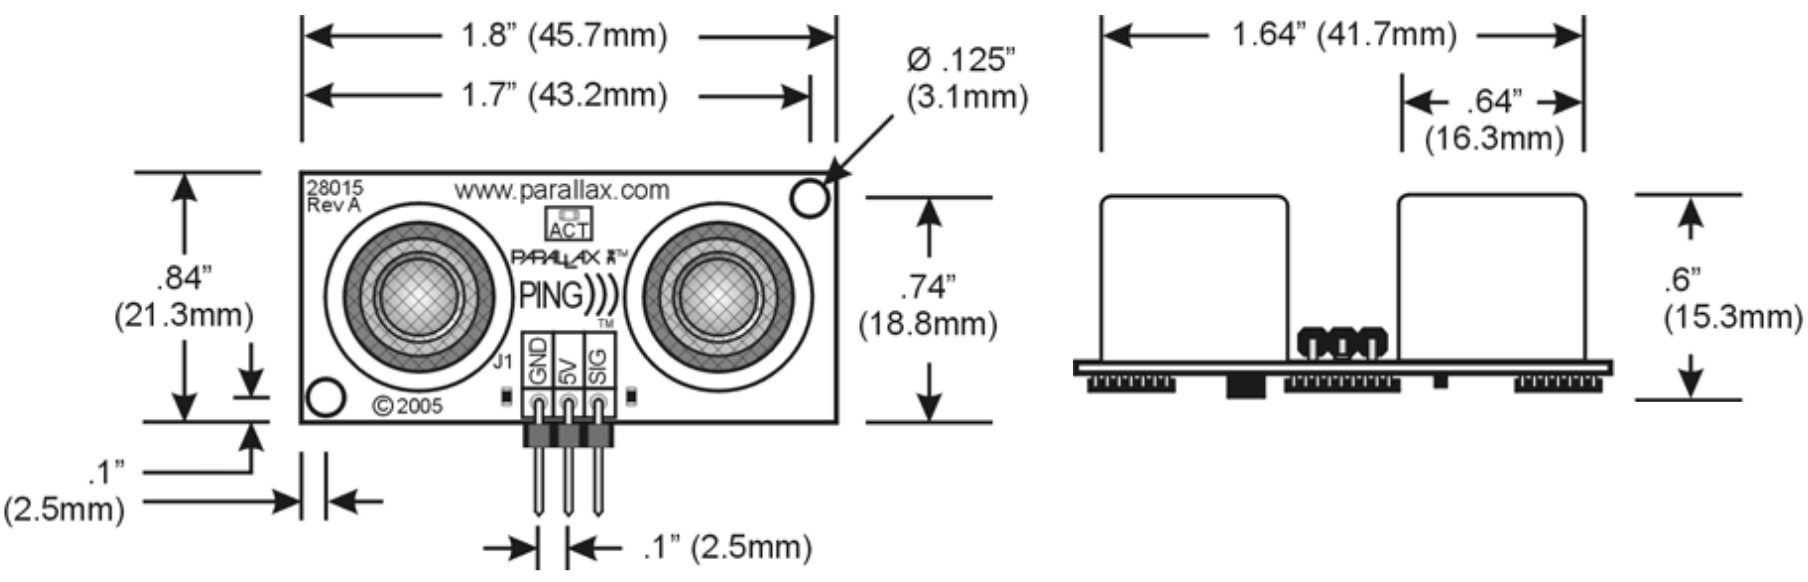
\includegraphics[width=0.75\linewidth]{./images/ping_dims.png}
        \centering
        \caption{Димензии на PING))) сензорот}
        \label{fig:ping_dims.png}
        \end{figure}

      \begin{figure}[H]
        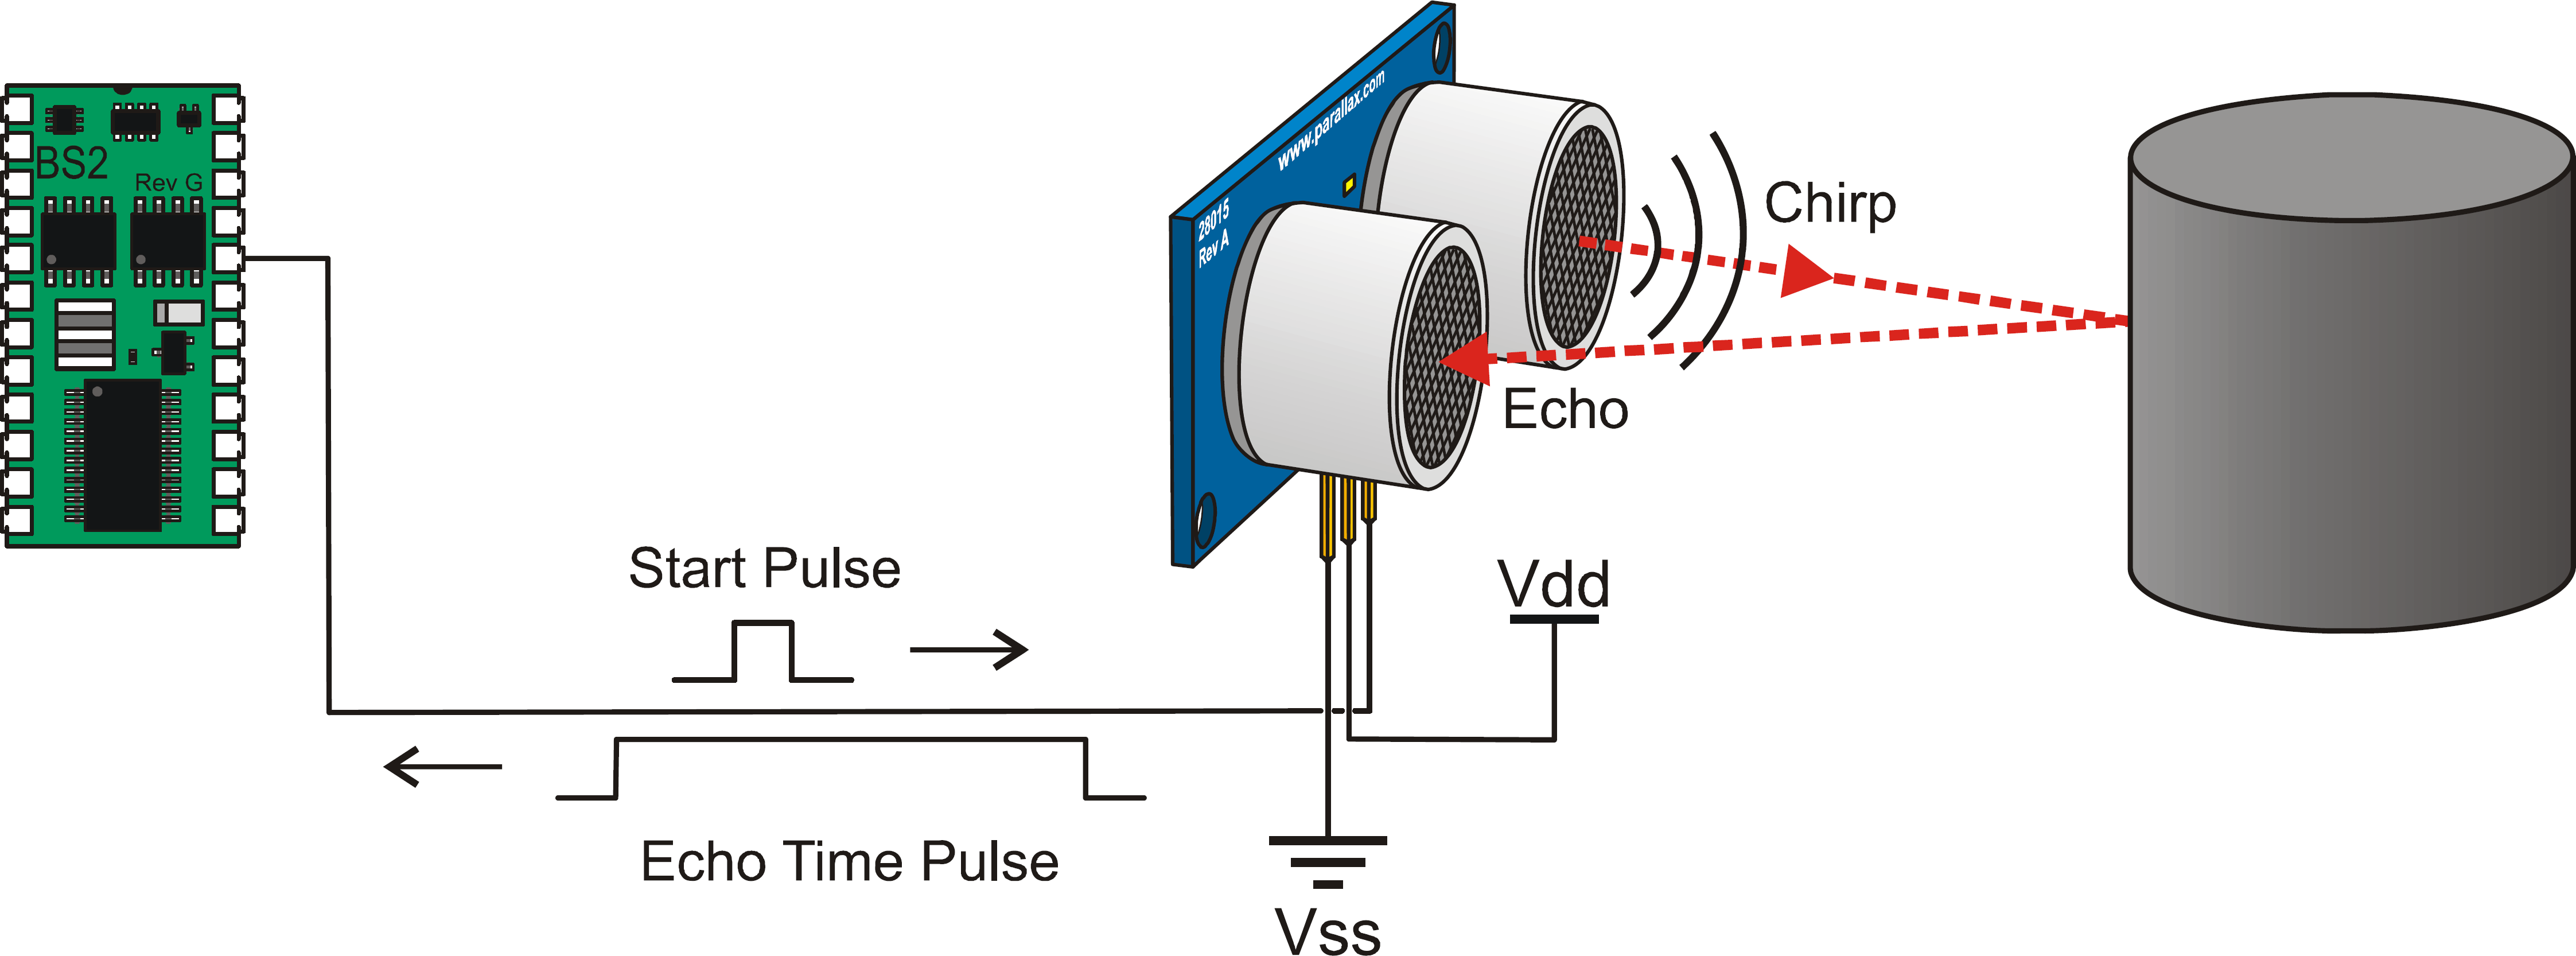
\includegraphics[width=0.75\linewidth]{./images/ping.png}
        \centering
        \caption{Шема и принцип на дејство на ултразвучен сензор}
        \label{fig:ping.png}
        \end{figure}

		  \paragraph{Протокол на комуникација\\}
        PING))) сензорот детектира предмети со емитирање на краток ултрасоничен збир (burst) на бранови, и потоа со „слушање“ за ехото. Под контрола на главен микроконтролер (пулс на активација), сензорот емитира краток 40kHz сигнал. Овој сигнал патува низ воздухот, се судира со објект и се одбива назад кон сензорот. Истовремено сензорот испраќа излезен пулс на микроконтролерот кој ќе се прекине штом се детектира ехото, кој всушност ни го дава растојанието до предметот(сл.\ref{fig:ping.png}).

      \begin{figure}[H]
        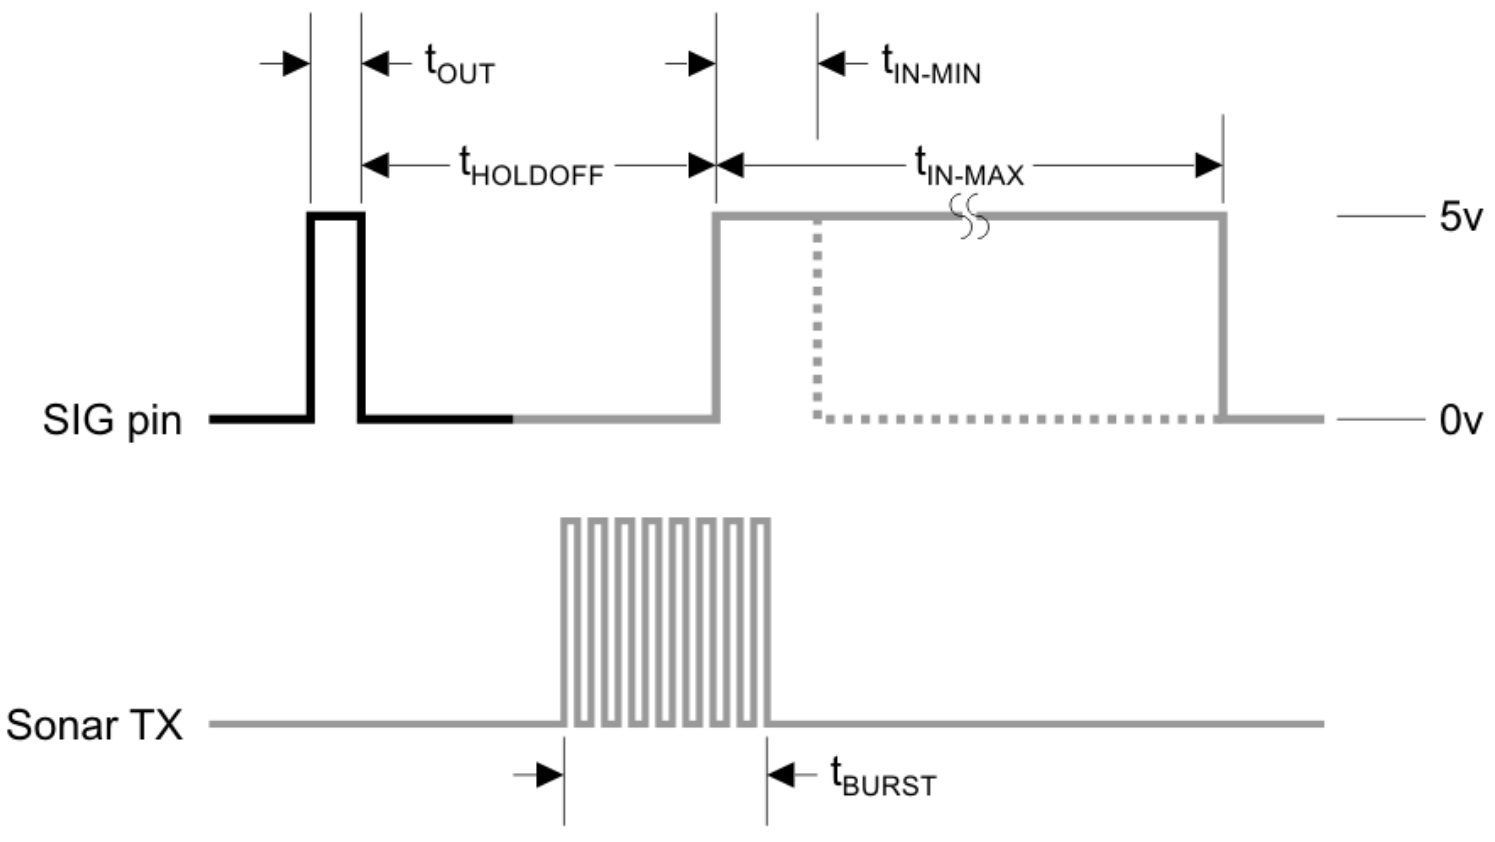
\includegraphics[width=0.75\linewidth]{./images/ping_sig.png}
        \centering
        \caption{Изглед на сигналот}
        \label{fig:ping_sig.png}
        \end{figure}

      \begin{table}[H]
        \caption{Карактеристики на сигналот}
        \label{tab:signalchar}
        \begin{center}
          \resizebox{\textwidth}{!}{
          \begin{tabular}{||c|l|l|l|l||}
            \hline
            Темна линија & Главен Уред & Влезен пулс на активација & $ t_{OUT} $ & $2\mu s$ (min), $5\mu s типично$ \\ \hline
            \multirow{5}{*}{Светла линија} & PING))) Сензор & Задржување на ехо & $ t_{HOLDOFF} $ & $750\mu s$ \\
            & & Фреквенција на сигналот (burst) & $ t_{BURST} $ & $ 200\mu s $ @ $ 40kHz $ \\
            & & Ехо повратен сигнал минимум & $ t_{IN-MIN} $ & $ 115\mu s $ \\
            & & Ехо повратен сигнал максимум & $ t_{IN-MAX} $ & $ 18.5\mu s $ \\
 						& & Пауза пред следно мерење & & $ 200\mu s $ \\
						\hline
          \end{tabular}}
          \end{center}
				\end{table}

      \paragraph{Позиционирање на објектот\\}
        PING))) сензорот не може прецизно да измери растојание до објект кој што:

      \renewcommand{\theenumi}{\alph{enumi}}
      \begin{enumerate}
        \item се наоѓа подалеку од 3m
        \item има мал агол на рефлектирачката површина со што сигналот нема да биде одбиен назад кон сензорот
        \item е премногу малечок за да рефлектира доволно звук назад кон сензорот
        \end{enumerate}

		  Дополнително, доколку PING))) сензорот е поставен на ниска позиција на уредот, има можност да детектира звук кој се одбива од подот.

      \begin{figure}[H]
        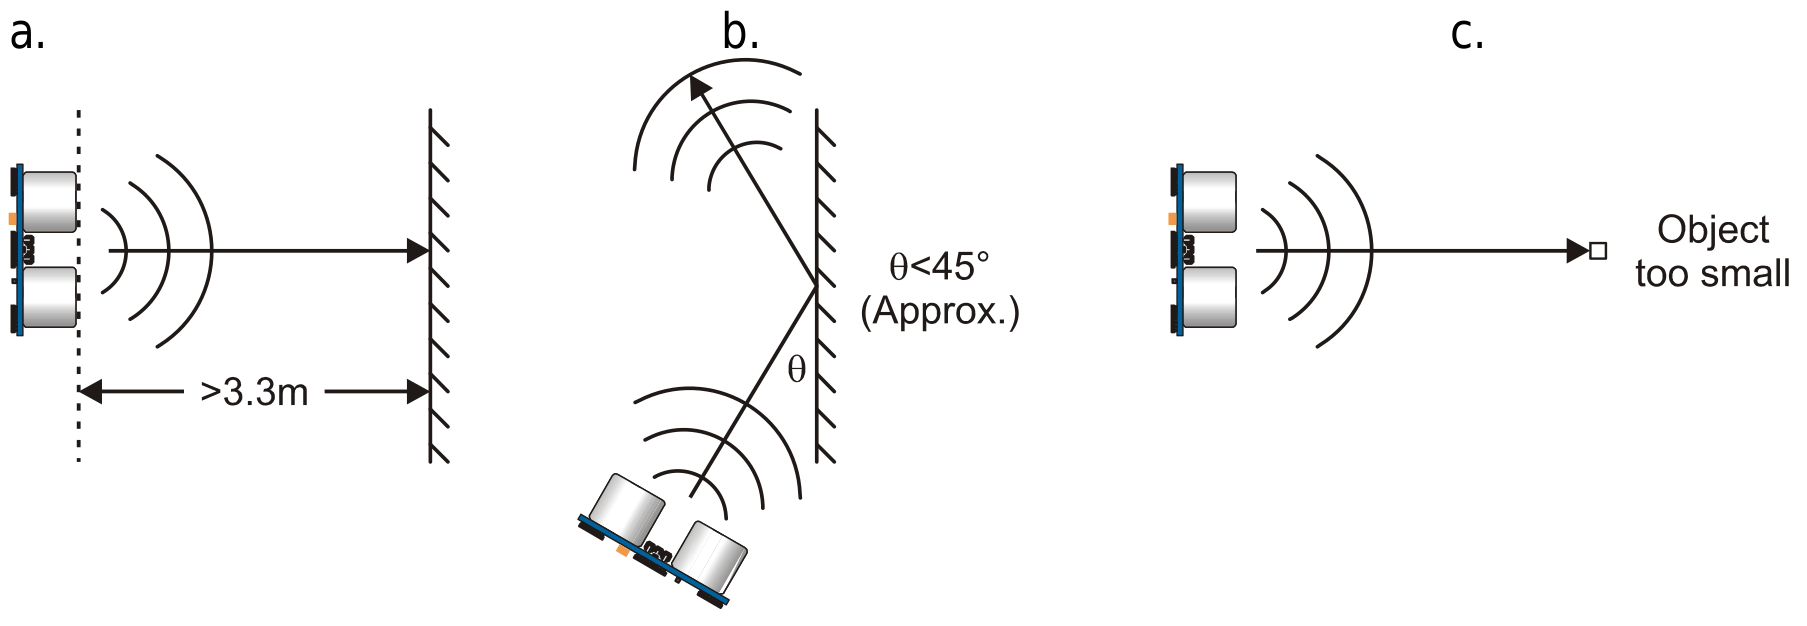
\includegraphics[width=0.75\linewidth]{./images/ping_obj.png}
        \centering
        \caption{Позиционирање на објектот}
        \label{fig:ping_obj.png}
        \end{figure}

\newpage

\section{NI sbRIO 9632}
	\begin{figure}[h]
		\centering
		\includegraphics[width=0.75\linewidth]{./images/sb_rio_1.png}
		\caption{sbRIO со обележани компоненти од \cite{experiments}}
		\label{fig:sb_rio_1.png}
		\end{figure}

  sbRIO (single-board Reconfigurable Input/Output) управувачките единици од National Instruments претставуваат компјутер монитран на една плочка (single board) наменета за случаи каде што е потребно решение со управување во реално време (Real Time). Оперативен систем кој работи во реално време (RTOS: Real Time Operating System) е изработен со особената цел да извршува функции кои барат големо ниво на временска прецизност и висок степен на надежност. За некој систем да се смета за RTOS, тој мора да има познато максимално време на извршување за секоја од неговите клучни операции. Системите кои можат сигурно да обезбедат максимален временски одѕив се вели дека работаат во потполно реално време, додека системите кои можат само понекогаш да обезбедат максимален временски одѕив се вели дека работаат во делумно реално време.

	Потребната брзина се постигнува со истовремето користење на FPGA чип и една обична микропроцесорска единица.

	sbRIO поседува 110 дигитални влезови/излези, 100 од кои се оспособени за PWM (Pulse Width Modulation), а 10 од кои се наменети за ниско-фреквентна намена. sbRIO поседува и 32 аналогни влезови, и 4 аналогни излези со ранг на излез од $ \pm 10\ V$ со $0.1\%$ грешка при типична употреба на $25\degree C \pm5\degree C$ \cite{sbrio}.

	sbRIO содржи и 3 сериски „С“ портови за поврзувањето на надворешни модули од NI за проширување на можностите на sbRIO да опфатат и актуација и аквизиција на податоци.

	\subsection{FPGA}
		Како што е објаснето во \cite{fpga}, FPGA, или „Field Programmable Gate Array“, претставува репрограмибилно интегрално коло кој поседува голем број на програмибилни логични порти. Кај обичните микроконтролери, логиката за управување се пишува и компајлира од некои програмски јазик како C, BASIC или некој графички јазик како G (LabVIEW). Во текот на овој процес се сублимираат во процесорски наредби/инструкции како ADD и MOV. Низата на можните наредби е единствена за секој микропроцесор. Кај FPGA колата, програмата не се сублимира на наредби, туку самата внатрешна архитектура на колото се подредува со електромагнетни полиња. Како резултат, се добива конфигурација на логични порти која ќе ја извршува задачата опишана во првобитната програма. Бидејќи FPGA-та нудат хардверско решение, нивното работење е често многу пати побрзо од работењето на обичните микроконтролери, но се подраги.

		\begin{figure}[h]
			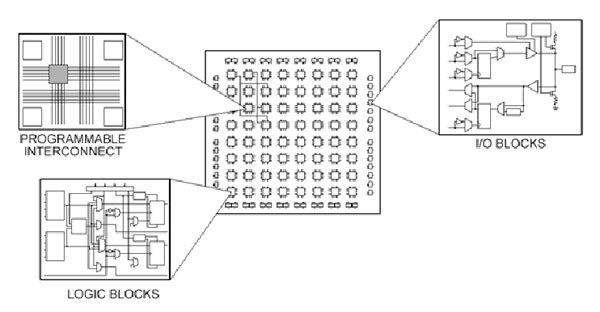
\includegraphics[width=0.75\linewidth]{./images/fpga_diagram.jpg}
			\centering
			\caption{Приказ на често сретнати термини кај FPGA кола од \cite{experiments}}
			\label{fig:fpga_diagram_jpg}
			\end{figure}

		FPGA колото што се наоѓа во sbRIO-то е моделот Xilinx Spartan 6, кој поседува 6 милиони репрограмибилни логични порти.

\newpage

\section{Теоретска Позадина}
  %Here we need:
  %\begin{enumerate}
    %\item Block Diagram of the Process DONEZO
    %\item Formal description of the sensor setup. i.e. Camera takes images, matches, detects bodies. DONEZO?
    %\item Describe our processing and selection based on various methods teleop/following
    %\item Section on mobile robotics, holonomicity, and differential drives
    %\item Section on the vector model and PD control DONEZO?
    %\end{enumerate}

  \subsection{Генерален Опис на Системот}
    \label{sec:general_desc}

    Започнувајќи од основната задача на системот, тој има цел да ги препознае личностите пред себе и според некои критериуми наложени од корисникот да одреди која личност најдобро соодветствува на тие критериуми. По тоа, роботот ќе ја следи избраната личност, одржувајќи некое одредено растојание. Брзината на моторите треба да биде доволно голема да се следи човекот со задоволителна брзина, а доволно мала за да не се појавуваат отскокнувања, нагли запирања, или осцилаторни движења.
    \begin{figure}[H]
      \centering
      \label{fig:final_form}
      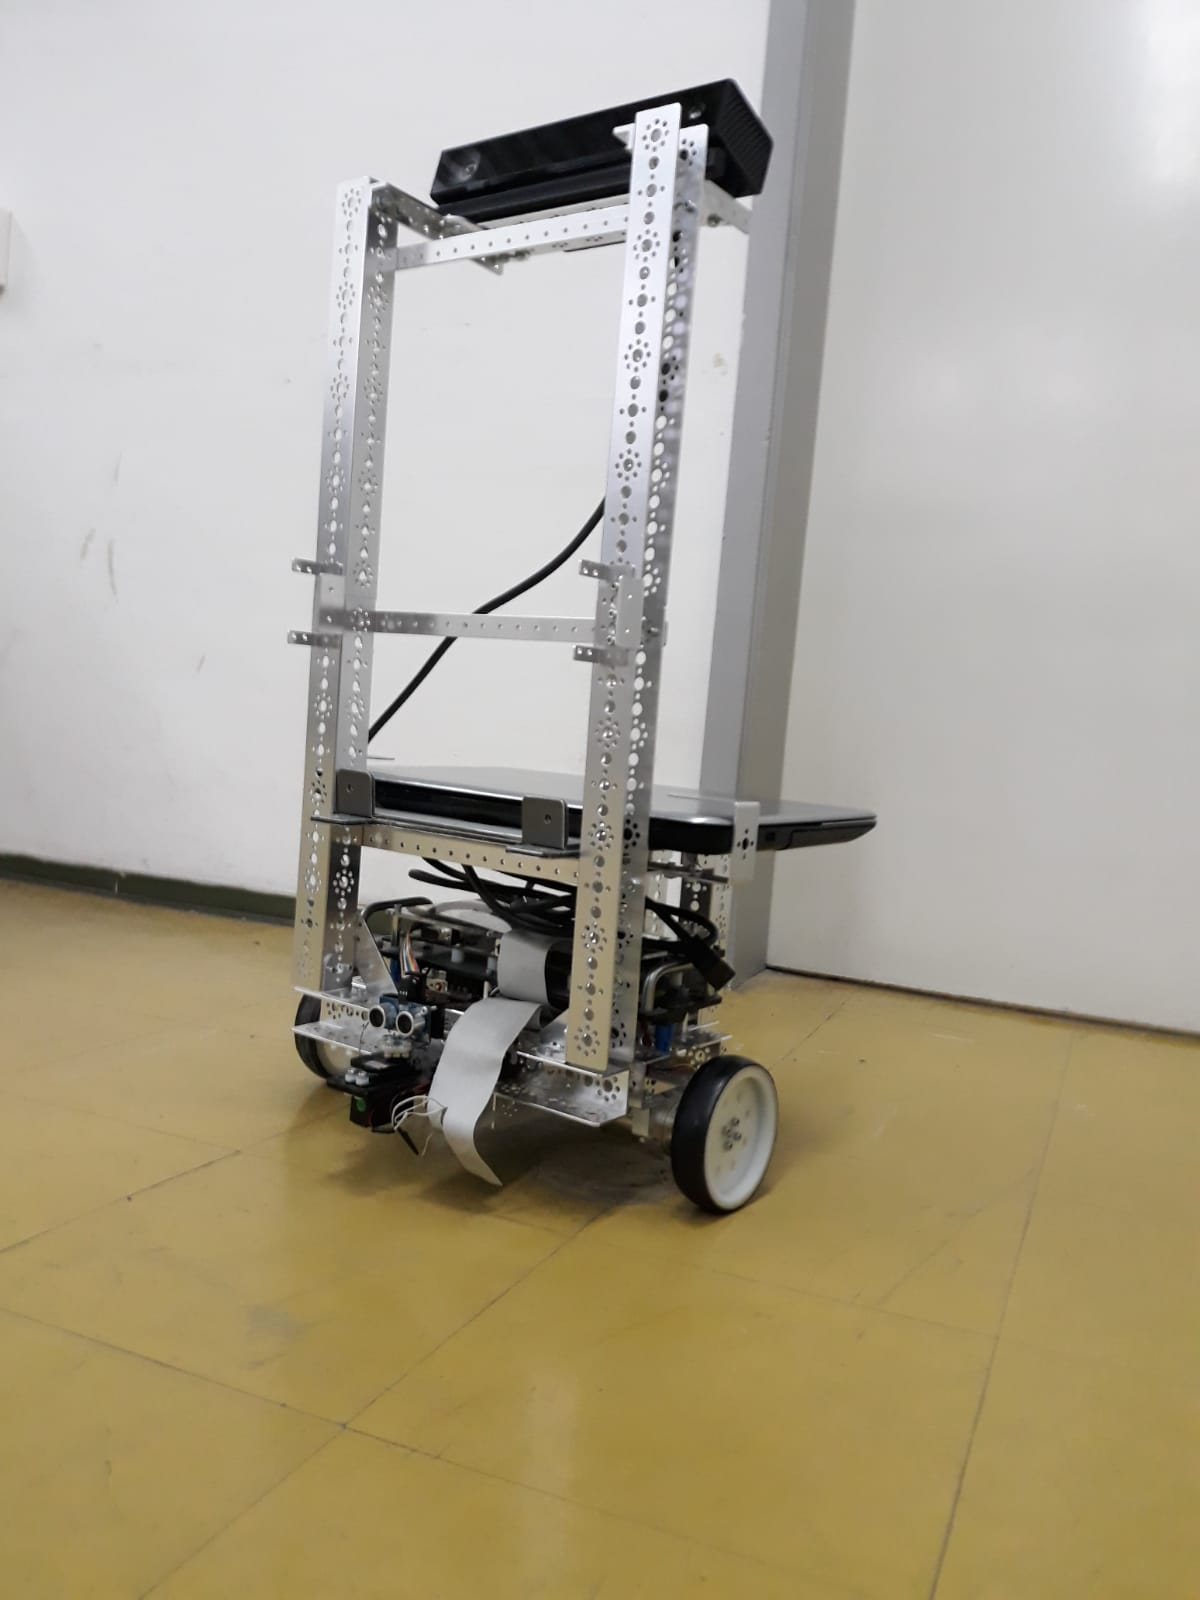
\includegraphics[width = 0.6\linewidth]{./images/final_form.jpeg}
      \caption{Крајната форма на DaNI}
    \end{figure}
    Системот се состои од длабинско-бојната камера Kinect од Microsoft и еден Robotics Starter Kit управуван со sbRIO едно-плочен компјутер, двата набавени од NI. Како главна процесорска единица се користи лаптоп кој го води целиот процес во LabVIEW. Како што се гледа при споредба на сл. \ref{fig:final_form} и сл. \ref{fig:dani_isometric}, роботот е прилично променет, и е веќе прилагоден кон задачата.

    Подолу се опишани во општи црти етапите на функционирање:
    \renewcommand{\theenumii}{\arabic{enumii}}
    \renewcommand{\theenumiii}{\arabic{enumiii}}
    \begin{enumerate}
      \item Kinect-от слика и испраќа бојна и длабинска информација за сцената пред себе со фреквенција од 30Hz кон главната процесорска единица.
      \item Со употреба на алгоритмите за човеково препознавање на Microsoft, се препознаваат луѓето кои се наоѓаат во сцената.
      \item Според критериумот за избор, една или нула од препознатите личности ќе биде избрана за следење, и нејзините декартови координати во однос на камерата се даваат на излез.
      \item Координатите се претворуваат во поларни координати и потоа уште еднаш се претворуваат во облик на општ информациски пакет и се испраќаат до едно-плочниот компјутер на роботот.
      \\
      Важно е да се опомени дека во меѓувреме разновидни процеси работаат паралелно, како што се читачи за промени во засилувањата на системот, посаканото растојание на роботот, и пораки за итно запирање на роботот.
      \item Роботот ги прима и толкува пораките, одредувајќи кој вид на информација го содржи тој пакет и која вредност ја носи. Во тек на обична употреба, роботот ќе ги прими поларните координати и ќе ги доведе во свој два паралелни ПД управувачи. Подетално ќе е разгледан двојниот-ПД систем во наредно поглавје.
      \item Излезите од ПД управувачите се претворуваат во дигитални PWM излези и се доведуваат до моторските управувачи.
      \end{enumerate}

  \subsection{Блок Дијаграм на Системот}
    Горенаведените елементи сочинуваат еден значително сложен систем, со развиени софтверски компоненти за управување на електромеханичкиот склоп што го претставува роботот. Иако системот е прилично сложен и со безбројно многу меѓузависности помеѓу информационите, електричните, и механичките потсистеми, за наша употреба самиот робот може да се упрости и да се апроксимира како механички систем од втор ред кој е линеарен и временски независен.\\

    \begin{figure}[h]
      \centering
      \begin{tikzpicture}
      \draw [->] (0,0) -- (1,0) node[above=0cm, pos=.2]{\small Реф.};
      %summer block
      \draw [thick] (1.25, 0)  circle (0.25cm) node{$\Sigma$} node[below left]{$-$} node[above left]{$+$};
      \draw [->] (1.25, -3) -- (1.25, -0.25);
      \draw [->] (1.5, 0) -- (2, 0) node[above = 0.02cm, pos=.5]{$\vec{x}$};
      \draw [thick](2, -0.75) rectangle (4.2, 0.75) node[above = 0.005cm,pos=.5]{LabVIEW} node[below = 0.05cm, pos=.5]{Управувач};
      \draw [->] (4.2, 0) -- (5, 0) node[above = 0.02cm, pos=.5]{V};
      \draw [thick] (5, -0.75) rectangle (7.2, 0.75) node[above = -0.1cm, pos=.5]{Моторски} node[below = 0.05cm, pos=.5]{Склоп};
      \draw [->] (7.2, 0) -- (8, 0) node[above = 0.05cm, pos=.5]{$\vec{\omega}$};
      \draw [thick] (8, -0.75) rectangle (9.5, 0.75) node[pos=.5]{$\dot x = \frac{\omega}{r}$};
      \draw [->] (9.5, 0) -- (10.5, 0) node[above = 0.05cm, pos=.5]{$\dot x$};
      \draw [thick] (10.5, -0.75) rectangle (11.5, 0.75) node[pos=.5]{\Large $\frac{1}{s}$};
      \draw [->] (11.5, 0) -- (13.5,0) node[above = -0.05cm, pos=.7]{$x\ (m)$};
      \draw [fill] (12,0) circle (0.05cm);
      \draw (12, 0) -- (12, -3);
      \draw [->] (12, -3) -- (8, -3);
      \draw [thick] (8, -3.75) rectangle (6, -2.25) node[pos=.5]{Kinect};
      \draw (6, -3) -- (1.25, -3);
      \end{tikzpicture}
      \caption{Блок дијаграм на усвоениот систем}
      \label{fig:blok_sema_real}
      \end{figure}

    Каде што:

    \begin{itemize}
      \item Реф. е референтното растојание на роботот кое што е побарано од корисникот.
      \item Векторот $\vec{x}$ ги претставува пропорционалните и диферецијалните компоненти на промената на растојанието.
      \item Блокот \textbf{LabVIEW Управувач} го претставува алгоритамот изведен во LabVIEW.
      \item $V$ е излезниот напон кој што се доведува до моторите.
      \item Излезот од моторите е $\omega = \theta/s$ во радијани.
      \item Излезот на претворувачкиот блок е брзината на роботот во $m/s$.
      \item По интегрирање со интеграторот $\frac{1}{s}$ се добива изминатиот пат на роботот во метри.
      \end{itemize}

  \subsection{Мобилна Роботика}
    Стационарните индустриски роботи во вид на роботски раце употребуваат во големо-сериското производство на автомобили дури од 1970тите \cite{robothistory}, каде што драстично ја подобрија продуктивноста во средини каде што работата е повторлива, бара голема прецизност, и/или е опасна.

    \bigbreak
    %Basically completely translated. I'd prefer to rework this
    Мобилните роботи би нашле - и наоѓаат ден денеска - примена во разновидни средини поради слични причини. Интелигентни и мобилни роботи можат да најдат примена во земјоделство, производство, болници, обезбедување, мерења во средини кои се штетни за човекот, како и безброј воени употреби \cite{robotics}.\\
    %we should ask viktor about words like that. He'll just choose one.
    Постојат разновидни елементи кои се применуваат за задвижување на роботите, како што се: нозе, тркала, и траки. Благодарение на модерните производни технологии и материјали, изводливи се начини на задвижување кои се моделирани на појави во природата (\textit{biomimicry}), како што се: перки, крилја, и нозе.

    \subsection{Холономност и диференцијален погон}
      Изборот на начинот на задвижување не се врши само согласно со условите на средината во која ќе функционира роботот, туку и со пресметковните ограничувања и потребите за агилно движење и степените на слобода. Тука се воведува концептот на \textbf{холономност} \cite{differential_drive_robots}. За робот се вели дека е холономен кога тој поседува можност за директно управување во секој од своите степени на слобода. Односно, рамнински робот (како DaNI) со три степени на слобода ($\theta,\ x,\ y$) е холономен ако тој има директна можност за задвижување по оска $x$, $y$, и да се ротира околу $\theta$. DaNI роботот, како и повеќето на роботи во класата на \textit{rovers} ја немаат оваа можност, бидејќи не можат директно да се преместуваат по оската $x$. Овие се нарекуваат \textbf{нехолономни}. За вакво хоризонтално движење, тие мораат да се ротираат, па по своја $y$-оска да се преместуваат додека не ја стигнат посаканата точка, и повторно да се заротираат кон точната ориентација.

      Бидејќи DaNI роботот има два мотори кои независно еден од друг се управуваат, имаме случај на диференцијален погон, каде што линеарната брзина ($\dot y$) е функција на големината на аголните брзини на моторите, додека аголната брзина ($\dot \theta$) е фунцкија на разликата на брзина помеѓу двата мотори. Во случај брзините на десното и левото тркало да се исти по големина а спротивни по знак, роботот би се ротирал вo место, додека еднакви брзини предизвикуваат задвижување нанапред. Секоја друга варијација на брзини предизвукува криволиниско движење по лак со радиус $R$ со центар наречен „моментален центар на ротација“ (МЦР). Равенките за пресметка на $R$, МЦР, и аголната брзина околу МЦР $\omega$ се \cite{differential_drive_robots}:
      $$ R = \frac{d}{2} \frac{v_d + v_l}{v_d - v_l} $$
      $$ {MCR} = [x - Rsin(\theta), y + Rcos(\theta)] $$
      $$ \omega = \frac{v_d - v_l}{d} $$
      Каде што:
      \begin{itemize}
        \item $d$ е меѓуосно растојание на тркалата
        \item $v_d$ е аголната брзина на десното тркало
        \item $v_l$ е аголната брзина на левото тркало
        \item $\theta$ е аголот создаден помеѓу осовините на тркалта и X-оската
      \end{itemize}

    \subsubsection{Вектор модел и ПД управување}
    \label{sec:doublePD}
      %recognize
      %find spots
      %return coords in m
      %calculate vectors (arg and mod)
      %compare vectors to setpoints
      %parallel PD controllers try to converge error on 0

      Откако камерата го препознае телото, таа ги наоѓа неговите карактеристичните точки, и ги преобразува нивните податоци од длабинската камера во $ x,y,z $ декардни координати во $ m $ каде што $ 0,0,0 $ е центарот на инфрацрвената камера, $x$ е хоризонталното растојание (лево и десно), $y$ е вертикалното растојание (горе и долу), и $z$ е нормалното растојание од камерата (напред и назад). Преку овие податоци, пресметуваме два вектори, т.е поларните координати - \textbf{аргумент} и \textbf{модулус}, каде што модулусот (\textit{mod}) е растојанието до карактеристичната точка на следеното лице, како што е прикажано на сликата и пресметката подолу.

      %INSERT IMAGE HERE CONTAINING A TOPDOWN VIEW OF THE CAMERA AND A PERSON, MAYBE ALSO A 2ND IMAGE WITH A FRONT VIEW.
      %      \begin{figure}[H]
      %        \includegraphics[width=0.55\linewidth]{./images/kinectView.png}
      %        \centering
      %        \caption{Поглед и координатен систем на камерата}
      %        \label{fig:kinectView.png}
      %        \end{figure}

      \begin{equation} \label{eq:cart2pol}
        \begin{aligned}
    	  mod = \sqrt{x^{2} + z^{2}} \\
        tan(arg) = \frac{x}{z} \\
        arg = tan^{-1}(\frac{x}{z})
        \end{aligned}
        \end{equation}

      Бидејќи најчесто сакаме личноста која што ја следиме да биде во центарот на видното поле на камерата, аргументот треба да се стреми кон вредност 0, додека модулусот треба да се стреми кон вредноста зададена од личноста која што се следи. Управувањето на овие два параметри го постигнуваме со два паралелни ПД управувачи. Едниот ПД управувач е одговорен за оддржување на аргумент 0, и на свој излез дава две инверзни брзини потребни за посаканата ротација, додека другиот ПД управувач е одговорен за модулусот и на излез дава две истонасочни брзини потребни за посаканот праволиниско движење.

      Поради апроксимацијата дека системот е линеарен и временски независен, двата излези од ПД управувачите можат едноставно да се соберат и да се доведе соодветниот напонски сигнал до моторите. Комбинацијата на чиста ротација и чисто праволиниско движење го произведува потребното криволиниско движење. Подолу се опишува целиот процес математички:

      $$      v_d^{rot} = K_p^{rot}(a_{ref} - a_i) + K_d^{rot}(a_i - a_{i-1}) $$
      $$      v_l^{rot} = -v_d^{rot}  $$
      $$      v_d^{lin} = v_l^{lin} = K_p^{lin}(m_{ref} - m_i) + K_d^{lin}(m_i - m_{i-1}) $$
      Според принцип на суперпозиција:
      $$      v_d = v_d^{rot} + v_d^{lin} $$
      $$      v_l = v_l^{rot} + v_l^{lin} $$
      Каде што:
      \begin{itemize}
        \item $a_i$ и $m_i$ се сегашните вредности на аргументот и модулусот
        \item $a_{i-1}$ и $m_{i-1}$ се претходните вредности на аргументот и модулусот
        \item $a_{ref}$ и $m_{ref}$ се референтите вредности за аргументот и модулусот
        \item $v_d^{rot}$ и $v_l^{rot}$ се ротацијоните брзини на десното и левото тркало
        \item $v_d^{lin}$ и $v_l^{lin}$ се линиските брзини на десното и левото тркало
        \item $K_p^{lin}$ и $K_p^{rot}$ се пропорционалните засилувања на линискиот и ротациониот ПД управувач
        \item $K_d^{lin}$ и $K_d^{rot}$ се диференцијалните засилувања на линискиот и ротациониот ПД управувач
        \item $v_d$ и $v_l$ се крајните брзини на десното и левото тркало
      \end{itemize}

      Во горенаведениот список, сите брзини се во $m/s$, сите агли се во радијани, и сите растојанија се во $m$.

  \subsection{Теорија на Боја за Компјутерски Системи}
    \label{sec:colour_theory}
    Во секојдневието, човекот ретко размислува за поимот боја. Објектите си имаат своја боја, и тоа е често крајот на приказната. Кога ќе се разгледа основната физика за бојата, поимот боја се разбира од гледна точка на електромагнетни бранови со посебни фреквенции. Оваа дефиниција е сосема задоволителна и исправна за инженерско размислување, но кога се дискутира за поимот на процесирање на слики станува многу важна уште една перспектива: претставувањето на една боја како три-димензионален вектор во еден конечен простор.
    \\
    Трихроматичната теорија на вид се појавила на почетокот на 18-тиот век, кога Томас Јанг преложил дека човековата способност да гледа бои била поради присуството на три различни видови на фотоприемнички клетки во очите \cite{young}. Теоријата била понатаму разработена од Џејмс Максвел и Херман вон Хелмхолц пред да биде физиолошки докажана од Гуннар Сваетчин во 1956-та година \cite{svaetchin}.
    \bigbreak
    Секои од овие клетки има способност да прима светлина со ниска (црвена), средна (зелена), или висока (сина) фреквентна содржина. Со суперпонирањето на информациите што ги добиваат секои од овие клетки се добива целосната бојна информација. Според овој модел, секоја боја може да се разреди во три елементарни компоненти: нејзината црвена (R), зелена (G), и сина (B) компонента. Овие компоненти можат да се ставаат во еден вектор $ V = [R\ G\ B]$. Човековото око може да препознае од прилика 10 милиони бои \cite{nColours}, што значи дека просторот во кој овој вектор би постоел е конечен. Ако се смета дека секоја од оските носи иста тежина, тие би имале иста максимална вредност. Ако се направи обид секоја компонента да се опише со еден бајт, произлегува максимална вредност во било која насока да е 255. Со таа максимална вредност, испаѓа дека целата боја се опишува со еден 24 битен број. Еден 24 битен број може да создаде $2^{24}$ = 16,777,216 комбинации. Од тука произлегува дека конечниот простор е коцка со димензии $a = R_{max} = G_{max} = B_{max} = 255 $, со максимален модулус на вектор $\sqrt{R_{max}^2 + G_{max}^2 + B_{max}^2}$, и со аргументски ограничувања по $\phi$ и $\gamma$ - $0 \leq \phi \leq \pi /2$, и $0 \leq \gamma \leq \pi /2$.
    \bigbreak
    \begin{figure}[h]
      \centering
      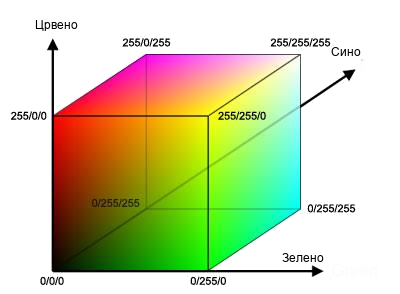
\includegraphics[width = 0.6\linewidth]{./images/colour_cube_mk.png}
      \caption{Конечниот боен простор од \cite{colourcube}}
      \label{fig:colour_cube_mk.png}

      \end{figure}

\newpage

\section{Софтверско управување со LabVIEW}
  LabVIEW (Laboratory Virtual Instrument Engineering Workbench) е софтверски пакет наменет за програмирањето на виртуелни уреди (инструменти) за мониторинг и управување на физички уреди. Инструментите што се програмираат во LabVIEW можат да се компајлираат и да се издаваат како комплетно независни програми кои можат да се монтираат како главен управувен софтвер на мехатроничките уреди и машини. LabVIEW инструментите се програмираат користејќи го нивниот сопствен графички програмски јазик, „G“.
  \\
  Основниот пакет на LabVIEW поседува многу од стандардните можности што се очекуваат од било кој програмерски јазик, како што се логички/булови операции, математички операции, и пристап до алатки за визуелизација на податоци.

  LabVIEW поддржува (и понекогаш бара) проширување со додатни пакети. На пример, овие пакети можат да содржат готови под-инструменти (sub-VIs) за обработка на сигнали (Signal Processing), или да овозможуваат соработка помеѓу LabVIEW и некои други технологии (FPGA module). Од овие пакети во оваа дипломска работа се употребени Real Time, FPGA, Vision Development, и Robotics пакетите. Првите два пакети го оспособуваат LabVIEW да програмира FPGA чипови и да управува во реално време, Vision Development олеснува оперирање со слики, додека Robotics пакетот содржи во себе голем број на готови инструменти за класична и инверзна кинематика, отчитување од сензори, и праќање наредби на моторите.
  \\
  Robotics пакетот исто поседува едно подмножество на инструменти наменети само за DaNI 2.0, и со тие е управуван DaNI роботот. Исто така, за посебна хардверска поддршка за Kinect и \textit{bluetooth} контролер од PlayStation се употребени библиотеките од \textit{LabVIEW MakerHub}.
  \\
  Да се спомени дека во контекстот на LabVIEW, термините \textit{функција} и \textit{блок} се земени за еднакви по значење, односно за меѓусебно заменливи.

  \subsection{Robotics модул: Starter Kit 2.0}
    Во Robotics модулот на LabVIEW, од интерес се готовите VIs за Starter Kit 2.0, кои содржат во нив потпрограми за иницијализација и деиницијализација на роботот и задавање на брзина на ротација на моторите. Тука се наброени и објаснети овие блокови.

		\paragraph{Иницијализација:\\}
			\begin{figure}[h]
				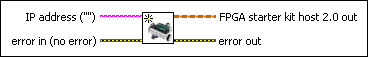
\includegraphics[width=0.55\linewidth]{./images/init.png}
				\raggedright
				\caption{VI за иницијализација}
				\label{fig:init.png}
				\end{figure}
		  Првиот блок служи за иницијализација на роботот. Како влез се доведува IP адресата на DaNI роботот, и според зададената адреса започнува комуникацијата со DaNI. При иницијализација на DaNI се создава „објект“ кој го претставува роботот. Програмерскиот термин „објект“ дефинира конгломерат на податоци и функции коj го опишува некој апстрактен предмет. Овие предмети се често неопипливи, но во случаи како нашиот, овој „објект“ е еден кибернетски претставнички меѓуслој кој ни овозможува комуникација со физичкиот систем во прашање. Како излез на оваа функција го добиваме објектот на DaNI, што ни претставува предуслов за употребата на било која од другите фунцкии. Error-in и error-out портите на VI-то се за заштита при некоја грешка во системот. Ако грешката е 1 (има грешка), целата функцијата на иницијализација се заменува со куса врска, и нема излезен објект.
      \\
      \textcolor[RGB]{150,150,150}{\rule{\linewidth}{1.6pt}}

    \paragraph{Деиницијализација:\\}
    	\begin{figure}[h]
        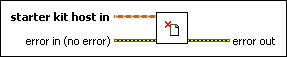
\includegraphics[width = 0.55\linewidth]{./images/deinit.png}
				\raggedright
				\caption{VI за деиницијализација}
				\label{fig:deinit.png}
				\end{figure}
      Овој блок се става на крај на програма за да се избрише објектот создаден од иницијализацијата, и да се направи соодветен излез. Без оваа крајна фунцкија, грешки се појавуваат при рестартирање на роботот и промени на програмата.\\
      \textcolor[RGB]{150,150,150}{\rule{\linewidth}{1.6pt}}

    \paragraph{Управување на моторите:\\}
      \begin{figure}[h]
        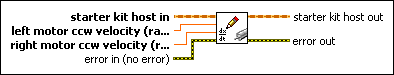
\includegraphics[width=0.55\linewidth]{./images/write_dc.png}
				\raggedright
				\caption{VI за дефинирање на брзина}
				\label{fig:write_dc.png}
				\end{figure}
			Овој блок е задолжен за управувањето на брзината на двата DC мотори на DaNI. За функционирањето на блокот потребен е самиот објект на DaNI, како и две вредности за врзините на моторите во \textit{rad/s}. За движење во било која насока, важно е да се опомени дека брзините на моторите морат да бидат со обратен предзнак порадни нивната обратна поставеност. Моторите имаат максимална брзина од 15.7 \textit{rad/s}.\\
      \textcolor[RGB]{150,150,150}{\rule{\linewidth}{1.6pt}}

    \paragraph{Отчитување од енкодерите:\\}
    	\begin{figure}[h]
        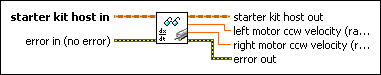
\includegraphics[width=0.55\linewidth]{./images/read_dc.png}
				\raggedright
				\caption{VI за отчитување од енкодерите}
				\label{fig:read_dc.png}
				\end{figure}

      Со овој блок се отчитуваат моменталните вредности од енкодерите на двата мотори на DaNI. Излезните вредности се во \textit{rad/s} и имаат \textit{double} формат, и заради тоа можат директно да се прикажат на \textit{indicator}, во \textit{chart} да се претставаат, или да се вклучат во други пресметки или контролери.\\
      \textcolor[RGB]{150,150,150}{\rule{\linewidth}{1.6pt}}

    \paragraph{Отчитување од ултразвучниот сензор:\\}
        \begin{figure}[H]
          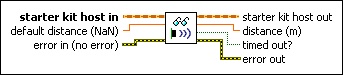
\includegraphics[width=0.55\linewidth]{./images/read_ping.png}
				  \raggedright
				  \caption{VI за отчитување од ултразвучниот сензор}
				  \label{fig:read_ping.png}
				  \end{figure}

        Овој блок служи за отчитување на информацијата дадена од ултразвучниот сензор, монтиран врз серво мотор на предниот дел од DaNI. Отчитаните вредности се исто во формат \textit{double} и се во мерна единица метри.\\
        \textcolor[RGB]{150,150,150}{\rule{\linewidth}{1.6pt}}

    \paragraph{Насочување на ултразвучниот сензор:\\}
    	\begin{figure}[H]
				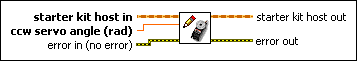
\includegraphics[width=0.55\linewidth]{./images/write_servo.png}
				\caption{VI за насочување на ултразвучниот сензор}
				\label{fig:write_servo.png}
				\raggedright
				\end{figure}

      Со овој блок се управува серво моторот на DaNI, односно се одредува поставеноста на ултразвучниот сензор. Блокот како влезови ги прима објектот на DaNI и посаканиот агол во радијани. Право пред роботот се смета за 0, позитивни вредности го вртат сензорот на лево, додека негативни вредности го вртат сензорот на десно. Доменот на сензорот е $ \pm \frac{\pi}{2}$, или $\pm 90 \degree$.\\
      \textcolor[RGB]{150,150,150}{\rule{\linewidth}{1.6pt}}

    Функцијата за отчитување од енкодерите недостига од програмата за следење. Ова е поради две причини. Првата причина е вградениот ПИД управувач во блокот за управување на моторите. Втората причина е тоа што самата повратна логика на управувањето - која ќе биде образложена понатаму - служи за корекција на било кои грешки или нелинеарности во самото физичко управување. Блокот е сепак споменат бидејќи се користи во една од стандардните програми на DaNI - Избегнување на пречки, која што е објаснета во поглавје \ref{sec:app1-avoidance}.

  \subsection{LabVIEW MakerHub модули}
    \subsubsection{Kinect модул}
      Модулот од NI MakerHub за отчитување од Kinect-от во LabVIEW ги сублимира во LabVIEW блокови сите функции за аквизиција на податоци кои што обично би се програмирале во јазик како C++ или C\#. Во оваа дипломска работа, од значење се следните фунцкии:

      \paragraph{Иницијализација:\\}
	      \begin{figure}[H]
	        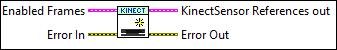
\includegraphics[width=0.55\linewidth]{./images/kinect_init_border.png}
	        \caption{VI за Иницијализација на Kinect-от}
		      \label{fig:kinect_init.png}
	        \raggedright
	        \end{figure}
        Слично како и кај блокот за иницијализација за роботот, оваа фунцкија на излез дава референции кон објектот што ја претставува самата камера, и сигнал на грешка. Во случајот на Kinect-от, нема потреба за доведување на било какви идентификациони информации ако се употребува само една камера.\\
        \textcolor[RGB]{150,150,150}{\rule{\linewidth}{1.6pt}}

      \paragraph{Деиницијализација:\\}
	      \begin{figure}[H]
	        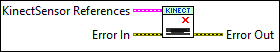
\includegraphics[width=0.55\linewidth]{./images/kinect_deinit_border.png}
	        \caption{VI за Деиницијализација на Kinect-от}
	        \label{fig:kinect_deinit.png}
	        \raggedright
	        \end{figure}
        Потполно исто со роботската деинцијализација, оваа функција ги прима референциите кон објектот и ги анулира, затворајќи ја комуникационата врска со камерата.\\
        \textcolor[RGB]{150,150,150}{\rule{\linewidth}{1.6pt}}

      \paragraph{Отчитување од Рамка:\\}
	      \begin{figure}[H]
	        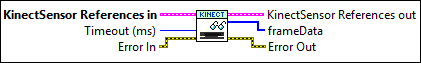
\includegraphics[width=0.55\linewidth]{./images/kinect_read_border.png}
	        \caption{VI за Отичитување на информација во рамка}
	        \label{fig:kinect_read.png}
	        \raggedright
	        \end{figure}
        Овој под-инструмент се нарекува и „полиморфски“ инструмент, бидејќи флексибилен е во однос на излезниот сигнал, без било какви промени на влезот. Оваа функција му дозволува на корисникот да одбери од која „рамка“ отчитува. Под рамка се подразбира вид на информација, односно избира корисникот да оберби бојна, длабинска, инфрацрвена, или „телесна“ слика. Важно е да се спомени дека телесната слика на излез не дава слика, туку низа со димензија $1 \times 6$ чиј секој елемент е податок од тип \textit{cluster} кој ги содржи координатите на телото во 3 разни координатни системи - бојна камера (т.е. пиксели), длабинска камера (т.е. пиксели), и вистинската камера (т.е. метри), како и некои други корисни мета-информации.\\
        \textcolor[RGB]{150,150,150}{\rule{\linewidth}{1.6pt}}

      \paragraph{Отчитување на Зглобни Координати:\\}
	      \begin{figure}[H]
	        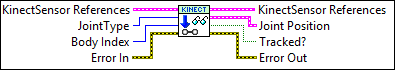
\includegraphics[width=0.55\linewidth]{./images/kinect_joints_border.png}
	        \caption{VI за Отчитување на зглобните координати на озбраната личност}
	        \label{fig:kinect_joints.png}
	        \raggedright
	        \end{figure}
        Функцијата за отчитување на координатите на самите зглобови ги прима како влез индексот од 0 - 5 на телото и една енумерирана вредност која го претставува самиот зглоб. Иако не се доведува низата што се генерира од отчитувањето на телесната слика, оваа фунцкија сепак има пристап до зглобовите. На излез го дава соодветниот \textit{cluster} на посаканиот зглоб.\\
        \textcolor[RGB]{150,150,150}{\rule{\linewidth}{1.6pt}}

    \subsubsection{PS4 контролер модул}
      MakerHub интерфејсот за PS4 контролерот овозможува лесно отчитување на податоци од сите копчиња и оски од PS4 контролер. Функционира според стандардната парадигма на LabVIEW, односно има блок за иницијализација, отчитување и деиницијализација, а има вградена можност за детекција на настани, т.е. промена на состојбата на копчињата.

      \paragraph{Иницијализација:\\}
	      \begin{figure}[H]
	        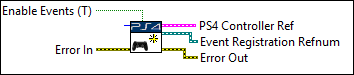
\includegraphics[width=0.55\linewidth]{./images/controller_init_border.png}
		      \caption{VI за Иницијализација на \textit{bluetooth} контролерот}
	        \label{fig:controller_init.png}
	        \raggedright
	        \end{figure}
        Стандарден блок за иницијализација на уред, во овој случај PS4 контролерот. По желба може да се избере дали да се иницијализира првиот конектиран уред, или во случај на повеќе уреди, може да се избере специфичен контролер по автоматски зададен индекс. Како излез од блокот повторно добиваме референции кон објектот, односно контролерот, и сигнал на грешка.\\
        \textcolor[RGB]{150,150,150}{\rule{\linewidth}{1.6pt}}

      \paragraph{Деиницијализација:\\}
        \begin{figure}[H]
	        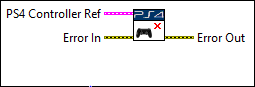
\includegraphics[width=0.55\linewidth]{./images/controller_deinit_border.png}
		      \caption{VI за Деиницијализација на \textit{bluetooth} контролерот}
	        \label{fig:controller_deinit.png}
	        \raggedright
	        \end{figure}
        Иста функција и влезови како и горенаведените блокови за деиницијализација.\\
        \textcolor[RGB]{150,150,150}{\rule{\linewidth}{1.6pt}}

      \paragraph{Отчитување:\\}
        \begin{figure}[H]
	        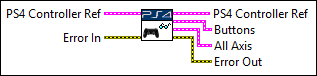
\includegraphics[width=0.55\linewidth]{./images/controller_read_border.png}
		      \caption{VI за отчитување на наредби од контролерот}
	        \label{fig:controller_read.png}
	        \raggedright
	        \end{figure}
        Оваа функција за отчитување има две излезни порти: првата порта има ги дава отчитуваните вредности на копчињата, а втората порта се користи за детекција на промени (\textit{Event Detection}) во состојбата на голем број од влезовите. Оваа порта понатаму се поврзува со \textit{Event Structure} и го поедноставува процесот на интегрирање на контролата во програмата.\\
        \textcolor[RGB]{150,150,150}{\rule{\linewidth}{1.6pt}}

  \subsection{Специјално изработени Виртуелни Инструменти и Контроли}
    \label{sec:bodydetect}
	  \begin{figure}[H]
	    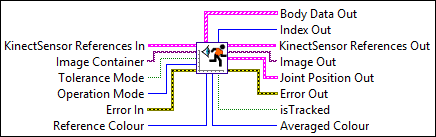
\includegraphics[width=0.55\linewidth]{./images/humanDetect_border.png}
		  \caption{Главен пресметковен VI за човеково препознавање и избор}
	    \label{fig:humanDetect.png}
	    \raggedright
	    \end{figure}

    \subsubsection{humanDetect}
      %\paragraph{humanDetect:\\}
      Функцијата \textit{humanDetect} служи за препознавање на човек и има два режими на операција. Првиот режим, наречен \textit{desperate} или \textbf{очаен}, ги дава на излез декартовите координати на првата личност која ќе биде детектирана.

      Вториот режим, наречен \textit{Colour Match} или \textbf{пребарување според боја}, врши избор на личност за следење според анализа бојата на претходно одредена област. Областа, во овој случај, претставува посебен полигон на пиксели што припаѓа на секоја од личностите. Оваа област може да се наоѓа било каде и да има било кој облик; во оваа функција, таа област се наоѓа во горниот дел (градниот кош) на човекот. Се проверува сличноста на овие области со некоја референта боја, и се избира за следење тој човек со најсоодветна обоена област. Анализата на овие области ќе биде подетално покриена во описите за други под-инструменти.\\
      \textcolor[RGB]{150,150,150}{\rule{\linewidth}{1.6pt}}

    \subsubsection{colourDist}
      %\paragraph{colourDist:\\}
	    \begin{figure}[H]
	      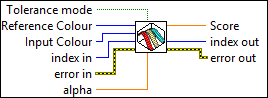
\includegraphics[width=0.55\linewidth]{./images/colourDist_border.png}
		    \caption{Потфункцијата \textit{colourDist} за обработка на бојна информација}
	      \label{fig:colourDist.png}
	      \raggedright
	      \end{figure}
      Подфункцијата \textit{colourDist} се наоѓа во инструментот за препознавање \textit{bodyDetect} и ја врши анализата на обоените области. Оваа фунцкија исто има два режими на работа со два вида на толеранти полиња на боја. На влез е доведена просечната боја на една област, и функцијата проверува дали оваа просечна боја припаѓа на едно претходно дефинирано толерантно поле, кое се наоѓа во дискретен тридимензионален боен декартов систем (поглавје \ref{sec:colour_theory}). Толерантното поле проверува за сличност според хроматичност (состав на боја), но и е проширено за да прифаќа еден поширок опсег на осветлувања.\\
      \textcolor[RGB]{150,150,150}{\rule{\linewidth}{1.6pt}}

      \paragraph{Режим - Толерантен цилиндар:\\}
        Првиот режим на работа поседува толерантно поле во облик на цилиндар, каде што радиусот на цилиндарот претставува „разлика во боен состав“ (односно хроматично отстапување), додека неговата висина го претставува опсегот на прифатени интензитети на осветленост. Толерантниот цилиндар како начин на споредба на бои е земен од трудот на К. Ким \cite{kim}. Сликовито е покажен овој режим подолу.

        Равенките за пресметка на хроматично отстапување, добиени од \cite{kim}, гласат:
        $$  \norm{\vec{x_t}}^2 = R^2 + G^2 + B^2,$$
        $$  \norm{\vec{v_{ref}}}^2 = R_{ref}^2 + G_{ref}^2 + B_{ref}^2, $$
        $$    (\vec{x_t} \cdot \vec{v_{ref}})^2 = R\ R_{ref} + G\ G_{ref} + B\ B_{ref} $$
        $$    colourDist(\vec{x_t}, \vec{v_{ref}}) = \delta = \sqrt{\norm{\vec{x_t}}^2 - \frac{(\vec{x_t} \cdot \vec{v_{ref}})^2}{\norm{\vec{v_{ref}}}^2}} $$
        \bigbreak

        Додека равенката за осветлувачко отстапување гласи:
        $$ \Delta I = \norm{\vec{x_t}} - \norm{\vec{v_{ref}} ци} $$
        \bigbreak
        Условот за припаѓање на некоја обоена област $i$ е:
        $$ \delta_{i} < \epsilon $$
        $$ I_{min}< \Delta I_i < I_{max} $$

        Каде $\epsilon$, $I_{min}$, и $I_{max}$ се константи зададени од програмерот.

        Доколку точката што ја претставува бојата (во декартовиот боен систем) припаѓа на овој цилиндар, личноста на која ѝ припаѓа оваа боја е ставена во низата на можни кандидати за следење.
        \begin{figure}[H]
          \centering
          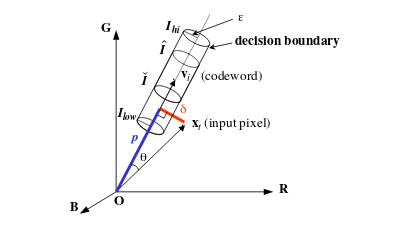
\includegraphics[width = 0.4\linewidth]{./images/cylinder.png}
          \caption{Графички приказ на толерантниот цилиндар од \cite{kim}}
          \label{fig:cylinder}
        \end{figure}

        Толерантниот цилиндар има мала толеранција при хроматични отстапувања, но е мошне толеранта на разлики во осветлување или интензитет, што значи дека подобро функционира во случаи каде осветлувањето може да се менува.

      \paragraph{Режим - Толеранта сфера:\\}
        Вториот режим на работа користи толерантно поле во облик на сфера, каде што нејзиниот волумен ги зафаќа и дозволениот боен состав и интензитет. Се пресметува тридимензионален вектор од просечната боја на доведената област до референтата боја, односно до центарот на сферата. Доколку овој вектор припаѓа целосно во сферата, личноста на која што ѝ припаѓа оваа боја станува кандидат за следење. Исто како и претходно, режимот е сликовито покажано подолу.

        Пресметката за релативниот вектор гласи:
        $$ \vec{V_i^r} = \vec{V_r} - \vec{V_i}= [R_r - R_i, G_r - G_i, B_r - B_i] $$
        Каде $\vec{V_i}$ е векторско прикажување на влезната боја, додека $\vec{V_r}$ е векторското претставување на референтната боја.
        Додека неговата должина (нормата $\norm{\vec{V_i^r}}$ ) се наоѓа со примена на питагорова теорема:
        $$ \norm{\vec{V_i^r}} = \sqrt{{R_i^r}^2 + {G_i^r}^2 + {B_i^r}^2} $$

        По споредување на бојните области на сите детектирани личности, сите кандитати за следење се сублимирани во една низа. Според видот на анализа, се наоѓа најзадоволителната (т.е. минималната) вредност на низата, и личноста на која ѝ припаѓа оваа вредност е избрана за следење. Во случај анализата да била цилиндрична, оваа вредност ќе биде хроматично отстапување, односно близина до оската на цилиндарот, занемарувајќи го осветлувањето. Доколку видот на анализа да бил сферичен, вредноста која се споредува е должината на векторот помеѓу центарот на сферата и влезната боја.
        \\
        Како излез на функцијата е индексот на личноста која треба да се следи.

        \begin{figure}[H]
          \centering
          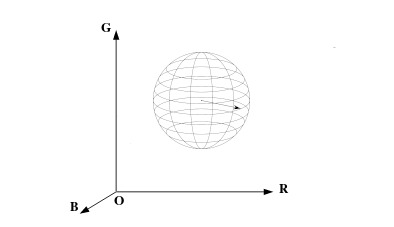
\includegraphics[width = 0.45\linewidth]{./images/sphere.png}
          \label{fig:sphere}
          \caption{Графички приказ на сферичното толеранто поле}
        \end{figure}
        Толерантата сфера, за разлика од цилиндарот, не е соодветен за употреба во ситуации со променливо осветлување. Бидејки сферата се шири во сите три димензии, таа има средна толеранција за осветлувачки разлики и средна толеранција на хроматично отстапување. Поради оваа, сферата е погодна за детекитрање на сложени нијанси на бои, особено при непрецизно човеково нагодување на бојата.

    \subsubsection{differentialDrive}
      %\paragraph{differentialDrive:\\}
	    \begin{figure}[H]
	      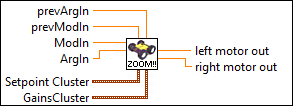
\includegraphics[width=0.55\linewidth]{./images/differential_drive_border.png}
		    \caption{Управувачот \textit{differentialDrive}}
	      \label{fig:diffDrive}
	      \raggedright
	      \end{figure}
      Блокот differentialDrive всушност го претставува главниот контролер во самиот систем, и го поседува двојниот ПД управувач претставен во поглавје \ref{sec:doublePD}. Тој на влез ги прима поларните координати на детектираната личност и на излез ги дава потребните вредности на брзини што требат да се впишат во моторите за да се постигне саканата положба, односно да конвергираат референтниот и реалниот вектор кон личноста.
      \\
      \textcolor[RGB]{150,150,150}{\rule{\linewidth}{1.6pt}}

    \subsubsection{Телеоперација}
      %\paragraph{Телеоперација:\\}
	    \begin{figure}[H]
	      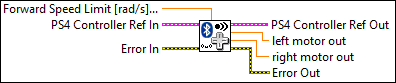
\includegraphics[width=0.55\linewidth]{./images/teleop_tooltip_border.png}
		    \caption{Блок за управување преку \textit{bluetooth}}
	      \label{fig:teleop}
	      \raggedright
	      \end{figure}
	    Блокот за телеоперација има интерфејс со блокот за отчитување на \textit{bluetooth} контролерот, кој на излез ги дава положбите на аналогните влезови и состојбите на бинарните влезови. Овие влезови се претворени преку аналоген-дигитален претворувач во 16 битен број, и потоа преку два специјално изведени управувачи во лининска брзина и сооднос на распределување на оваа брзина помеѓу двата мотори, односно овозможување на попрецизна контрола и движење со влезови различни од минималните и максималните вредности.\\
      \textcolor[RGB]{150,150,150}{\rule{\linewidth}{1.6pt}}

    \subsubsection{Typedefs}
      \label{sec:typedefs}
      Во програмата се појави потреба на засебно групирање на податоци во определени структури (односно \textit{clusters}). Овие структури претставуваат логични собири на податоци, како на пример информации за засилувањата или брзините на моторите. Исто е важно да овие структури да се строго дефинирани, унифицирани преку целиот софтвер. Согласно овие барања произлегоа \textit{typedefs}, односно композитни информации со одредени дефиниции кои можаат да се повикаат на сличен начин како обичните типови на податоци како што се \verb+int32+ и \verb+double+ \cite{lvforeveryone}.

      \paragraph{Засилувања:\\}
	      \begin{figure}[H]
	        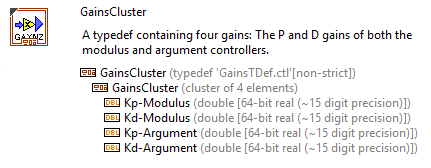
\includegraphics[width=0.55\linewidth]{./images/typedef_gains_border.png}
		      \caption{Typedef за засилувања}
	        \label{fig:gain_typedef}
	        \raggedright
	        \end{figure}
        Typedef-от за засилувања ги содржи четирите засилувања потребни за двојниот ПД управувач: пропорционални и диференцијални засилувања за управување и на модулусот и на аргументот.\\
        \textcolor[RGB]{150,150,150}{\rule{\linewidth}{1.6pt}}

      \paragraph{Брзини:\\}
	      \begin{figure}[H]
	        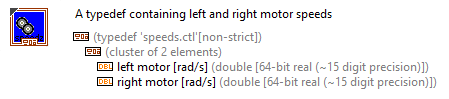
\includegraphics[width=0.55\linewidth]{./images/typedef_speeds_border.png}
		      \caption{Typedef за брзини}
	        \label{fig:gain_typedef}
	        \raggedright
	        \end{figure}
	      Овој typedef ги содржи конкретните брзини на моторите, кои се праќаат до роботот при режим на телеоперација.\\
        \textcolor[RGB]{150,150,150}{\rule{\linewidth}{1.6pt}}

      \paragraph{Референтни Вредности:\\}
	      \begin{figure}[H]
	        \includegraphics[width=0.55\linewidth]{./images/typedef_setpoints_border.png}
		      \caption{Typedef за референтни вредности}
	        \label{fig:setpoints_typedef}
	        \raggedright
	        \end{figure}
	      Референтните вредности се содржат во облик на горенаведениот typedef.\\
        \textcolor[RGB]{150,150,150}{\rule{\linewidth}{1.6pt}}

      \paragraph{Стопирање на Роботот:\\}
	      \begin{figure}[H]
	        \includegraphics[width=0.55\linewidth]{./images/typedef_stop_border.png}
		      \caption{Typedef за стопирање на роботот}
	        \label{fig:setpoints_typedef}
	        \raggedright
	        \end{figure}
        Typedef-от за сопирање на роботот содржи само еден \textit{boolean}, но сепак е корисен при употребата на мрежен тек (поглавје \ref{sec:message_handler}).\\
        \textcolor[RGB]{150,150,150}{\rule{\linewidth}{1.6pt}}

      \paragraph{Порака:\\}
        \begin{figure}[H]
          \includegraphics[width=0.85\linewidth]{./images/typedef_message.png}
          \caption{Typedef за пораки}
          \label{fig:message_typedef}
          \raggedright
          \end{figure}
        Можеби најважниот typedef, пораката содржи два елементи: еден блок општа меморија кој може да содржи било кој вид на инфомација (\textit{variant}, и етикета која кажува кој вид на информација е во варијантата. Ова е многу корисно бидејќи ја отстранува потребата за повеќе од еден мрежен тек - понатаму образложено во поглавје \ref{sec:message_handler}.

  \subsection{Образложение на Софтверот}

    \begin{figure}[H]
      \centering
      \includegraphics[width = 0.75\linewidth]{./images/pineapple_summer.png}
      \label{fig:pineapple}
      \caption{Главниот интерфејс за корисници на програмата, со видео од што гледа роботот}
    \end{figure}
    Следи изведбата во LabVIEW на етапите на функционирање опишани во поглавје \ref{sec:general_desc}. Програмата се состои од два софтвери кои работат паралелно на две соседни машини: персоналниот компјутер (главна процесорска единица) и вградениот sbRIO компјутер на DaNI роботот. На главната единица работат повеќе паралелни \textit{while} рутини, како што се:

    \paragraph{Произведувачи на Параметри:\\}
      Три произведувачи на параметарски пораки се состојат во една настанска структура, чекајќи да се зададе промена на некој параметар од страна на корисникот и да се постави новата информација на челото на редот за пораки кои ќе се праќаат до роботот.
      \begin{figure}[H]
          \centering
          \includegraphics[width=0.75\linewidth]{./images/gain_message_generator.png}
          \caption{Произведувач на Пораки - Засилувања}
          \end{figure}
      \begin{figure}[H]
          \centering
          \includegraphics[width=0.75\linewidth]{./images/setpoint_message_generator.png}
          \caption{Произведувач на Пораки - Рефентни Вредности}
          \end{figure}
      \begin{figure}[H]
          \centering
          \includegraphics[width=0.75\linewidth]{./images/robot_stop_generator.png}
          \caption{Произведувач на Пораки - Запирање на Роботот}
          \end{figure}
      Овие произведувачи работат во настанска структура (\textit{event structure}) \cite{lvforeveryone}, односно реагираат само кога ќе има промена во таа вредност за која се одговорни.

    \paragraph{Произведувач на движечки наредби:\\}
      Произведувачот на движечки наредби е главниот дел од програмата, и во зависност од режимот на работа одбран од корисникот, тој функционира на различни начини. Доколку корисникот избере режим на телеоперација, роботот се управува со \textit{bluetooth} контролерот како било кое друго возило со радио управување. Доколу корисникот избере еден од режимите на автономна работа, роботот ќе ја изврши соодветната функција (поглавје \ref{sec:bodydetect}), при која на излез ќе добие соодветни наредби за движење.
      \begin{figure}[H]
        \centering
        \includegraphics[angle=-90, scale=0.75]{./images/command_generator_true.png} %FIX THIS IMAGE
        \caption{Произведувач на наредби при автономно движење}
        \end{figure}
      Независно од тоа како се добиени овие наредби, тие се пакуваат во формата на општата порака и се поставуваат во редот за пораки.
      \begin{figure}[H]
        \centering
        \includegraphics[width=0.8\linewidth]{./images/command_generator_false.png}
        \caption{Произведувач на наредби при телеоперација}
        \end{figure}

    \bigbreak

    \paragraph{Управувач на Пораки:\\} %Управувач на пораки наместо управувач
      \label{sec:message_handler}
      Сите пораки се ставени во еден ред на податоци, создаден со \textit{Queue} фунцкијата. Секој произведувач ги става своите пораки во овој ред. Наредбите за движење се ставаат на крајот на редот, додека другите се сметаат за итни и се ставаат на челото на редот. Структурата за раковедење со пораките има за задача да ги отчитува пораките од челото на редот и да ги испраќа преку мрежниот тек (\textit{Network Stream}) до роботот. Мрежниот тек е комуникациски интерфејс кој припаѓа на LabVIEW, и поради тоа тој има поддршка за сите негови видови на податоци, вклучувајќи и \textit{typedefs}. Тоа значи дека, за разлика од поопшти комуникациски протоколи како TCP/IP и UDP, овој протокол нема потреба од припрема на податоци пред испраќање, ниту посебно толкување при примање.

      \begin{figure}[H]
        \centering
        \includegraphics[width=0.35\linewidth]{./images/message_handler.png}
        \caption{Управувачот на пораки}
        \end{figure}

      Но, еден недостаток е тоа што секој мрежен тек може да пренесува само еден вид на податок, пр. \verb+uint16+ или \verb+string+. За ова да се заобиколи, се употребува специјалниот typedef \textbf{порака} (поглавје \ref{sec:typedefs}). Поради структурата податок-етикета, пораката може да се прилагоди за пренесување на било кој вид на податок (вклучувајќи и други typedefs), и на овој начин со еден мрежен тек се пренесуваат сите посакани податоци.

    \paragraph{Толкувач на \textit{Bluetooth} Наредби:\\}
      Со употреба на погоре споменатите библиотеки и една настанска структура, се толкуваат податоците од контролерот, како што се промената на режим и итното застанување и прекинување на роботот.

      Со притискање на триаголник копчето на контролерот, во настанската структура се препознава промена на состојбата на тоа копче, и со тоа, преку логиката вршиме инкрементација на енумератор-от задолжен за пратење на режимот на работа. При тоа:

      \begin{itemize}
        %\setlength\itemsep{-0.5em}
        \item TeleOp соодветствува на вредност 0 и претставува почетна (односно \textit{default} режим),
        \item Desperate соодветствува на вредност 1,
        \item ColourMatch соодветствува на вредност 2.
        \end{itemize}

      \begin{figure}[H]
        \centering
        \includegraphics[width=0.75\linewidth]{./images/mode_switch.png}
        \caption{Толкувач на \textit{Bluetooth} Наредби}
        \end{figure}

      Кога енумераторот (во овој случај пратен со локална променлива) достигне вредност која соодветствува на ColourMatch, тогаш се ресетира на почетната вредност.

      Исто така, во настанската структура се вклучени и две други копчиња, \textit{Share} и \textit{Options}, кои соодветно се користат за стопирање на програмата на компјутерот и програмата на роботот. При тоа треба да се внимава роботот да биде првиот којшто ќе биде запрен, бидејќи командата за запирање се испраќа преку мрежниот тек.

    \paragraph{Читач на рачни гестикулации:\\}
      Рутината за отчитување на рачни гестикулации е активна во секој циклус, меѓутоа врши отчитување само во циклуси во кои е препознаена и се следи личност. Индексот на таа личност се користи како показател за да се добијат информациите за состојбата на телото на таа личност. Од нив, се користи само податокот за состојбата на левата дланка, т.е \textit{HandLeftState}. Овој податок има три можни вредности, но во оваа рутина се користат само отворена (\textit{Open}) и затворена (\textit{Closed}) состојба.

      \begin{figure}[H]
        \centering
        \includegraphics[width=0.85\linewidth]{./images/hand_control.png}
        \caption{Читач на рачни гестикулации}
        \end{figure}

      Во зависност од состојбата на левата дланка, се врши или инкрементација или декрементација на референтното растојание кое треба да се оддржува до личноста која се следи. Инкрементацијата и декрементацијата се со вредности од $0.025m$ при секој успешен циклус.
    \bigbreak
    Во оваа работа, роботот всушност ги има полесните задачи. Задачата на роботот е да ги прими пораките што му стигнуваат преку мрежниот тек, да ги толкува, и да одлучи како да се однесува според содржината на тие пораки.

    \paragraph{Читач на пораки:\\}
    Читачот на пораки има задача да ги прими пораките, кои се во формат на „порака“ typedef (поглавје \ref{sec:typedefs}), и да ги разреди во своите две компненти - етикетата и содржината.
      \begin{figure}[H]
        \centering
        \includegraphics[width=0.85\linewidth]{./images/robot_msg.png}
        \caption{Читач на пораки}
        \label{fig:parser}
        \end{figure}
    Етикетата на пораката е енумерирана вредност што е исто еден typedef - односно флексибилно се додаваат и одземуваат етикети. Енумерацијата содржи во неа по една етикета/вредност за секој можен вид на податок што може да стигне од компјутерот до роботот. Оваа етикета се доведува до одлучувачот (\textit{case selector}) на читачот - прикажан на сл. \ref{fig:parser} - и според тоа функцијата \textit{variant to data} ќе ја толкува содржината на доведената информација на соодветен начин.
\newpage


\section{Анекс I - Избегнување пречки со хистограм на векторски-полиња} %REPLACE VFH IMAGES WITH BETTER QUALITY ONES.
  \label{sec:app1-avoidance}
  Методот на хистограм со векторски полиња (ХВП) се состои од намалување (кратење) на податоци во две фази, наспроти постарите техники кои користат само еден чекор во кратење на податоци. Постојат три нивоа на претставување на податоци:

  \begin{enumerate}
    \item Највисокото ниво содржи детален опис за околината во која се наоѓа роботот. Во ова ниво, дво-димензионалниот Cartesian хистограм (С) се надополнува со нови податоци во реално време.
    \item Второто, средишно ниво е едно димензионален поларен хистограм (Н) кој се гради околу моменталната локација на роботот. Н содржи n аголни сектори со одредена ширина.
    \item Последното ниво, најниското ниво, од претставување на податоци е излезот од ХВП алгоритамот.
    \end{enumerate}

  За разлика од другите програми, имплементацијата на ХВП во LabVIEW користи само локален поларен хистограм, а не и Cartesian хистограмот. Овој недостаток е исправен со вградување на енкодерот од кој што се црпат информации за далечина и правец.

  Најпрво се генерира дво-димензионален хистограм околу роботот, што ги претставуваат пречките, чии што информации се добиваат од сензорот. Вториот чекор е конверзијата на дво-димензионалниот во едно-димензионален хистограм и потоа во поларен хистограм. Најпосле, алгоритамот го означува најдобриот сектор со ниски поларни вредности, и ги пресметува аголот и брзината за да се постигне тој правец.

  \begin{figure}[H]
    \centering
    \includegraphics[width=0.35\linewidth]{./images/2d_his.png}
    \caption{Конструкција на 2D хистограм}
    \label{fig:2d_his.png}
    \end{figure}

  \begin{figure}[H]
    \centering
    \includegraphics[width=0.35\linewidth]{./images/1d_his.png}
    \caption{Репрезентација на 1D хистограм}
    \label{fig:1d_his.png}
    \end{figure}

  Принципот на работа е всушност избирање најголема празнина преку податоците од поларниот хисторграм, од каде што се пресметуваат правецот, насоката и оддалеченоста.

  \begin{figure}[H]
    \centering
    \includegraphics[width=0.5\linewidth]{./images/vfh_lv.png}
    \caption{ХВП блок во LabVIEW}
    \label{fig:vfh_lv.png}
    \end{figure}

  Влезовите \textit{Distances} и \textit{Direction angles} се добиваат од податоците кои што ги отчитува сензорот. \textit{Distances} е низа од податоци за далечините на пречките. \textit{Direction angles} аналогно е низа со агли кои што започнуваат од центарот на сензорот до секоја од далечините (аглите десно од центарот се означени како позитивни а оние лево од центарот како негативни вредности). \textit{Distance threshold} е влез кој што дефинира незначителни пречки односно роботот игнорира објекти кои што се на далечина поголема од зададениот \textit{distance threshold}.

  При тоа, објектите кои што ги детектира сензорот кои се наоѓаат на растојание и агол помали од \textit{panic threshhold distance} и \textit{panic threshhold angle} кои го состојат \textit{panic range} влезот се идентификуваат како област на околината која што треба да се избегне.

  Излезот \textit{nearest obstacle} е структура од податоци која се добива како група од два елементи - агол и растојание до најблиската пречка. Блок дијаграмот на ХВП е даден на сл.\ref{fig:vfh_block_diagram.png}.

  \begin{figure}[H]
    \includegraphics[width=0.75\linewidth]{vfh_block_diagram.png}
    \centering
    \caption{Блок дијаграм на Алгоритам за Избегнување}
    \label{fig:vfh_block_diagram.png}
    \end{figure}

  За да се одреди дали одредена далечина претставува празнина или пречка, секој елемент се става во \textit{loop} со индексирање при што се врши споредба со distance threshold. Имаме булов излез (1 или 0) при што 0 се доделува на далечини кои што се поголеми од distance threshold, а 1 доколку не се. Резултатот е низа со нули и единици која што се менува како што роботот се движи. Споредбата на излезите е влез во Case Structure. Ако вредноста на моменталната празнина е подобра од минатата, се јавува \textbf{true} со што новата празнина станува најдобра и е новиот излез, а ако е обратно добиваме \textbf{false} каде што претходните податоци на големина и офсет (реден број на вредноста во низа) се најдобра празнина и се сеуште излез.

  Со овие податоци, роботот се насочува и движи кон најдобрата детектирана празнина.
\newpage
\section{Анекс II - Линкови до Github страни на изворните кодови}
    На следниот линк може заинтересираниот читач да го најде целосиот код за примерот од поглавјe \ref{sec:example}. Кодот е напишан во C++ во Visual Studio 2017 Community и има потреба од openCV библиотеката, како и SDK-то на Kinect-от.

    https://github.com/markogalevski/DaNI\_Kinect2\_Tracker
    \\
    Целата програма за дипломската работа напишана во LabVIEW 2012 може да се спушти од следниот линк.

    https://github.com/markogalevski/Bachelors-LabVIEW

    Потребно e корисникот да ги има следните пакети:
    \begin{itemize}
      \item OS: $\geq$ Windows 8
      \item LabVIEW 2012 (32bit)
      \item LabVIEW Robotics модул
      \item LabVIEW FPGA модул
      \item LabVIEW Real-Time модул
      \item LabVIEW Vision Development модул
      \item LabVIEW NI RIO Drivers
      \item $\geq$.NET4.0
      \item Kinect 2.0 SDK
      \item VI Package Manager - MakerHub Kinect 2 и MakerHub PS4 Controller модули
      \end{itemize}

\medskip
\nocite{*}
\newpage
\printbibliography[heading=bibintoc,title={Користена литература}]

\end{document}
